% 英文で執筆する場合はクラスファイルへのオプションを[T,E]としてください.
% If you want to write your paper in English, pass to [T,E] options to document class.
\documentclass[T,J]{fose} % 「コンピュータソフトウェア」用のクラスファイルは compsoft です.
\taikai{2023} % 固定です.出版委員長が毎年変更してAuthor Kitを配布してください.

\usepackage [dvipdfmx] {graphicx}
\usepackage{multirow}
\usepackage{caption}

% ユーザが定義したマクロなどはここに置く.ただし学会誌のスタイルの
% 再定義は原則として避けること.

% 以下は説明のために使用したパッケージであるため,削除可能.
\usepackage{fancyvrb}
\usepackage{xurl}
\usepackage{cite}
\usepackage{color}
\usepackage{graphicx}
\usepackage{ascmac}
\usepackage{textcomp}
% \usepackage[dvipdfmx]{color} クラッシュしていてなくても動くのでコメントアウト


\newcommand{\todo}[1]{\colorbox{yellow}{{\bf TODO}:}{\color{red} {\textbf{[#1]}}}}
\newcommand{\done}[2]{\colorbox{green}{{\bf DONE}:} {\textbf{[#1]}}}
\newcommand{\checked}[3]{\colorbox{red}{ここまでチェック済み}}

\begin{document}

% 論文のタイトル
\title{Scratchにおけるプログラム類似度とオブジェクト\\動作軌跡類似度の分析}
% 以下の \etitle(と\@etitle)はFOSE論文フォーマット独自のマクロです.
% FOSEに投稿した論文を発展させてコンピュータソフトウェアに投稿される場合はコメントアウトしてください.
% \setetitleは奇数ページのヘッダに表示する文字列(\etitle)を設定するためのマクロです.
% タイトルが2行に渡る場合は "\\" を 使用することで任意の位置で改行をすることができます.
\setetitle{An Analysis of Program Similarity and Object Motion Trajectory Similarity between Scratch Works}
%\setetitle{Long Long Long Long Long Long \\ Long Long Long Long Long \\ Long Long Long Long Long Long Long Long Long Long Long Long Paper Title}

% タイトル,著者などが複数行にわたり,論文冒頭の著者名が日本語アブストと重複して描画された場合に以下のコメントアウトを外してください.
%\longtitle

% 著者
% 和文論文の場合,姓と名の間には半角スペースを入れ,
% 複数の著者の間は全角スペースで区切る
%
\author{岡本 圭悟 伊原 彰紀
%
% ここにタイトル英訳 (英文の場合は和訳) を書く.
% 英語タイトルは論文1ページ目左下,著者らの名前・所属一覧の一番上に表示される
%
% 上記\setetitle中で改行した場合は "\etitle" を削除し,改行(\\)を入れていないタイトルを記載してください.
% \ejtitleは1ページ目左下に挿入されるタイトルとして使用されます.
% また,"\etitle"はFOSE論文フォーマット独自のマクロです.
%\ejtitle{\etitle}
%
% ここに著者英文表記 および
% 所属 (和文および英文) を書く.
% 複数著者の所属はまとめてよい.
%
% 複数著者の所属は以下のようにまとめてよい.
\shozoku{Keigo Okamoto, Akinori Ihara}{和歌山大学システム工学部}
{Faculty of Systems Engineering, Wakayama University}
}

%
% 和文アブストラクト
% In English paper, content of Jabstract will be ignored. 
\Jabstract{
ビジュアルプログラミング言語Scratchでは,ユーザが制作した作品をオンライン上に公開することができ,また公開された作品を検索することで,実装の参考にすることができる.ただし,検索結果にはユーザが期待するオブジェクト動作を含まない作品,期待するオブジェクト動作を含むが作品によって実装方法が異なることも多い.一方で,プログラムは類似していてもオブジェクト動作が異なることもある.このようなプログラムの類似性とオブジェクト動作の類似性の乖離は,Scratchにおけるプログラミング検索における作品の収集の妨げになることが示唆される.本研究では,Scratchにおいて制作されるプログラムの類似度の測定手法,およびオブジェクト動作軌跡の類似度の測定手法を提案し,プログラムの類似性とオブジェクト動作軌跡の類似性の乖離を明らかにする.ケーススタディとして4,000件のScratch作品を対象に,プログラムが類似するか否か,オブジェクト動作軌跡が類似するか否かの4種類に分類した結果,プログラムは類似するがオブジェクト動作軌跡が類似しない作品は全体の約1\%,オブジェクト動作軌跡は類似するがプログラムが類似する作品は全体の約28\%存在することを確認した.
}
%
% 英文アブストラクト(本サンプルの原論文にはなし)
%\Eabstract{
%\todo{英文アブスト}
%}
%
\maketitle \thispagestyle {empty}
%%%%%%%%%%%%%%%%%%%%%%
\section{はじめに}
%%%%%%%%%%%%%%%%%%%%%%
プログラミング的思考の育成を目的とし,我が国を含め世界中でプログラミング教育を本格的に推進している.特に,ビジュアルプログラミングは,画像オブジェクトの移動や効果音の制御など,命令処理を持つブロックを組み合わせることで直観的にプログラムの実装をおこなうことができるため,プログラミング初学者に広く利用されている.プログラミング的思考の育成に,ビジュアルプログラミング言語を用いた教育が有効であることが明らかにされている\cite{Sugiura2008}\cite{Mori2011}\cite{Dasgupta_2016}.ビジュアルプログラミングのオンライン開発環境であるScratchは世界中の教育機関やプログラミング教室で利用されている.
%杉浦学,松澤芳昭,岡田健,大岩元.アルゴリズム構築能力育成の導入教育:実作業による概念理解に基づくアルゴリズム構築体験とその効果.情報処理学会論文誌,Vol.49,No.10,pp.3409-3427,2008.
%森秀樹, 杉澤学, 張海, 前迫孝憲.Scratchを用いた小学校プログラミング授業の実践 : 小学生を対象としたプログラミング教育の再考(教育実践研究論文).日本教育工学論文誌,Vol.34, No.4, pp.387\UTF{2013}394, 2011.

Scratchでは,ユーザは制作したプログラム作品にタイトルや作品の説明文を付けてScratchのオンラインサービス上に公開することができ,2023年7月時点には1億3500万件\footnote{Scratch Statistics: \url{https://scratch.mit.edu/statistics/}}以上の作品が公開されている.Scratchは公開済みの作品を対象に自然言語による作品検索サービスを提供しており,公開済み作品の中からユーザが制作したい作品,実現したい動作を検索し,実装の参考にしている\cite{Resnick_2009}.
%Mitchel Resnick, John Maloney, Andr´es Monroy-Hern´andez, Natalie Rusk, Evelyn Eastmond, Karen Brennan, Amon Millner, Eric Rosenbaum, Jay Saul Silver, Brian S Silverman, Yasmin Bettina Kafai, Scratch: Programming for all, Communications of the ACM, Vol.52, No.11, pp.60-67, 2009.
Scratchで制作する作品は小規模なプログラムが多く,使用するブロックも限られているため,検索によって類似するプログラムを含む作品が多数出力される.その一方で,プログラムは類似していてもオブジェクトの動作が異なることもある.このようなプログラムの類似性とオブジェクト動作の類似性の乖離は,Scratch上のプログラミング検索における作品の収集の妨げになることが示唆される.

本研究は,Scratchにおけるプログラムが類似する作品とオブジェクトの動作軌跡が類似する作品の違いを分析するために,Scratchにおいて制作されるプログラムの類似度の計測方法,およびオブジェクトの動作軌跡の類似度の計測方法を提案する.プログラムの類似度の計測方法にはプログラムの編集距離を用いる(3章).オブジェクトの動作軌跡の類似度の計測方法には動的時間伸縮法(DTW: Dynamic time warping)を用いる(3章).本研究では,ケーススタディとしてScratchAPIを用いて時系列順に収集し,条件に基づいてフィルタリングした4,000件の作品を対象に,プログラムが類似するか否か,オブジェクトの動作軌跡が類似するか否かの4種類に分類し,それぞれの作品の特徴を分析する.

続く\ref{sec:RelatedWork}章では本論文の立ち位置を説明するための関連研究と研究動機を述べる.\ref{sec:Similarity}章では本論文で用いる類似度の測定手法を述べる.\ref{sec:Analysis}章ではケーススタディで用いるデータセットとアプローチ,その結果と考察を述べ,\ref{sec:con}章で本研究をまとめる.

%%%%%%%%%%%%%%%%%%%%%%
\section{Scratchにおける作品間の類似度}\label{sec:RelatedWork}
%%%%%%%%%%%%%%%%%%%%%%

\subsection{ビジュアルプログラミング言語Scratch}\label{subsec:Scratch}

ScratchはMITメディアラボが開発するビジュアルプログラミング言語の開発環境であり,ユーザはプログラムの命令処理を持つブロックを組み合わせ,画像オブジェクトの移動や効果音の入出力などをプログラムで制御することによりゲームやアニメーションなどの作品を制作できる.図\ref{fig:Scratch-description}は,Scratchにおける作品制作画面を示す.Scratchにおける作品は主にブロック,スクリプト,スプライトの3つの要素で構成される.
\begin{itemize}
\item ブロック:プログラムを構成する最小の単位であり,それぞれ特定の命令処理を持つ.ユーザは図\ref{fig:Scratch-description}に示すようなブロックを組み合わせることでプログラムを実装する.Scratchでは,画像の移動を制御する座標移動ブロック,条件分岐や繰り返しなどの制御ブロックなどを提供しており,種類に応じて役割,色,形が異なる.
\item スクリプト:図\ref{fig:Scratch-description}に示すように複数のブロックを組み合わせて制作したプログラムを指す.特に,スクリプトの先頭にはプログラムを開始するイベントブロックを使用し,スクリプトを開始するためのトリガーを設定する.同じイベントブロックを持つスクリプトが並列に存在する場合は,同時にスクリプトを実行開始することができる.
\item スプライト:図\ref{fig:Scratch-description}に示すように作品中に使用する画像オブジェクトを指す.各スプライトには,一つ以上のスクリプトが紐づいており,スプライトは実行画面上で,スクリプトに含まれる命令処理の通りに動作する.
\end{itemize}
%--------------------
\begin{figure}[t]
	\centering
	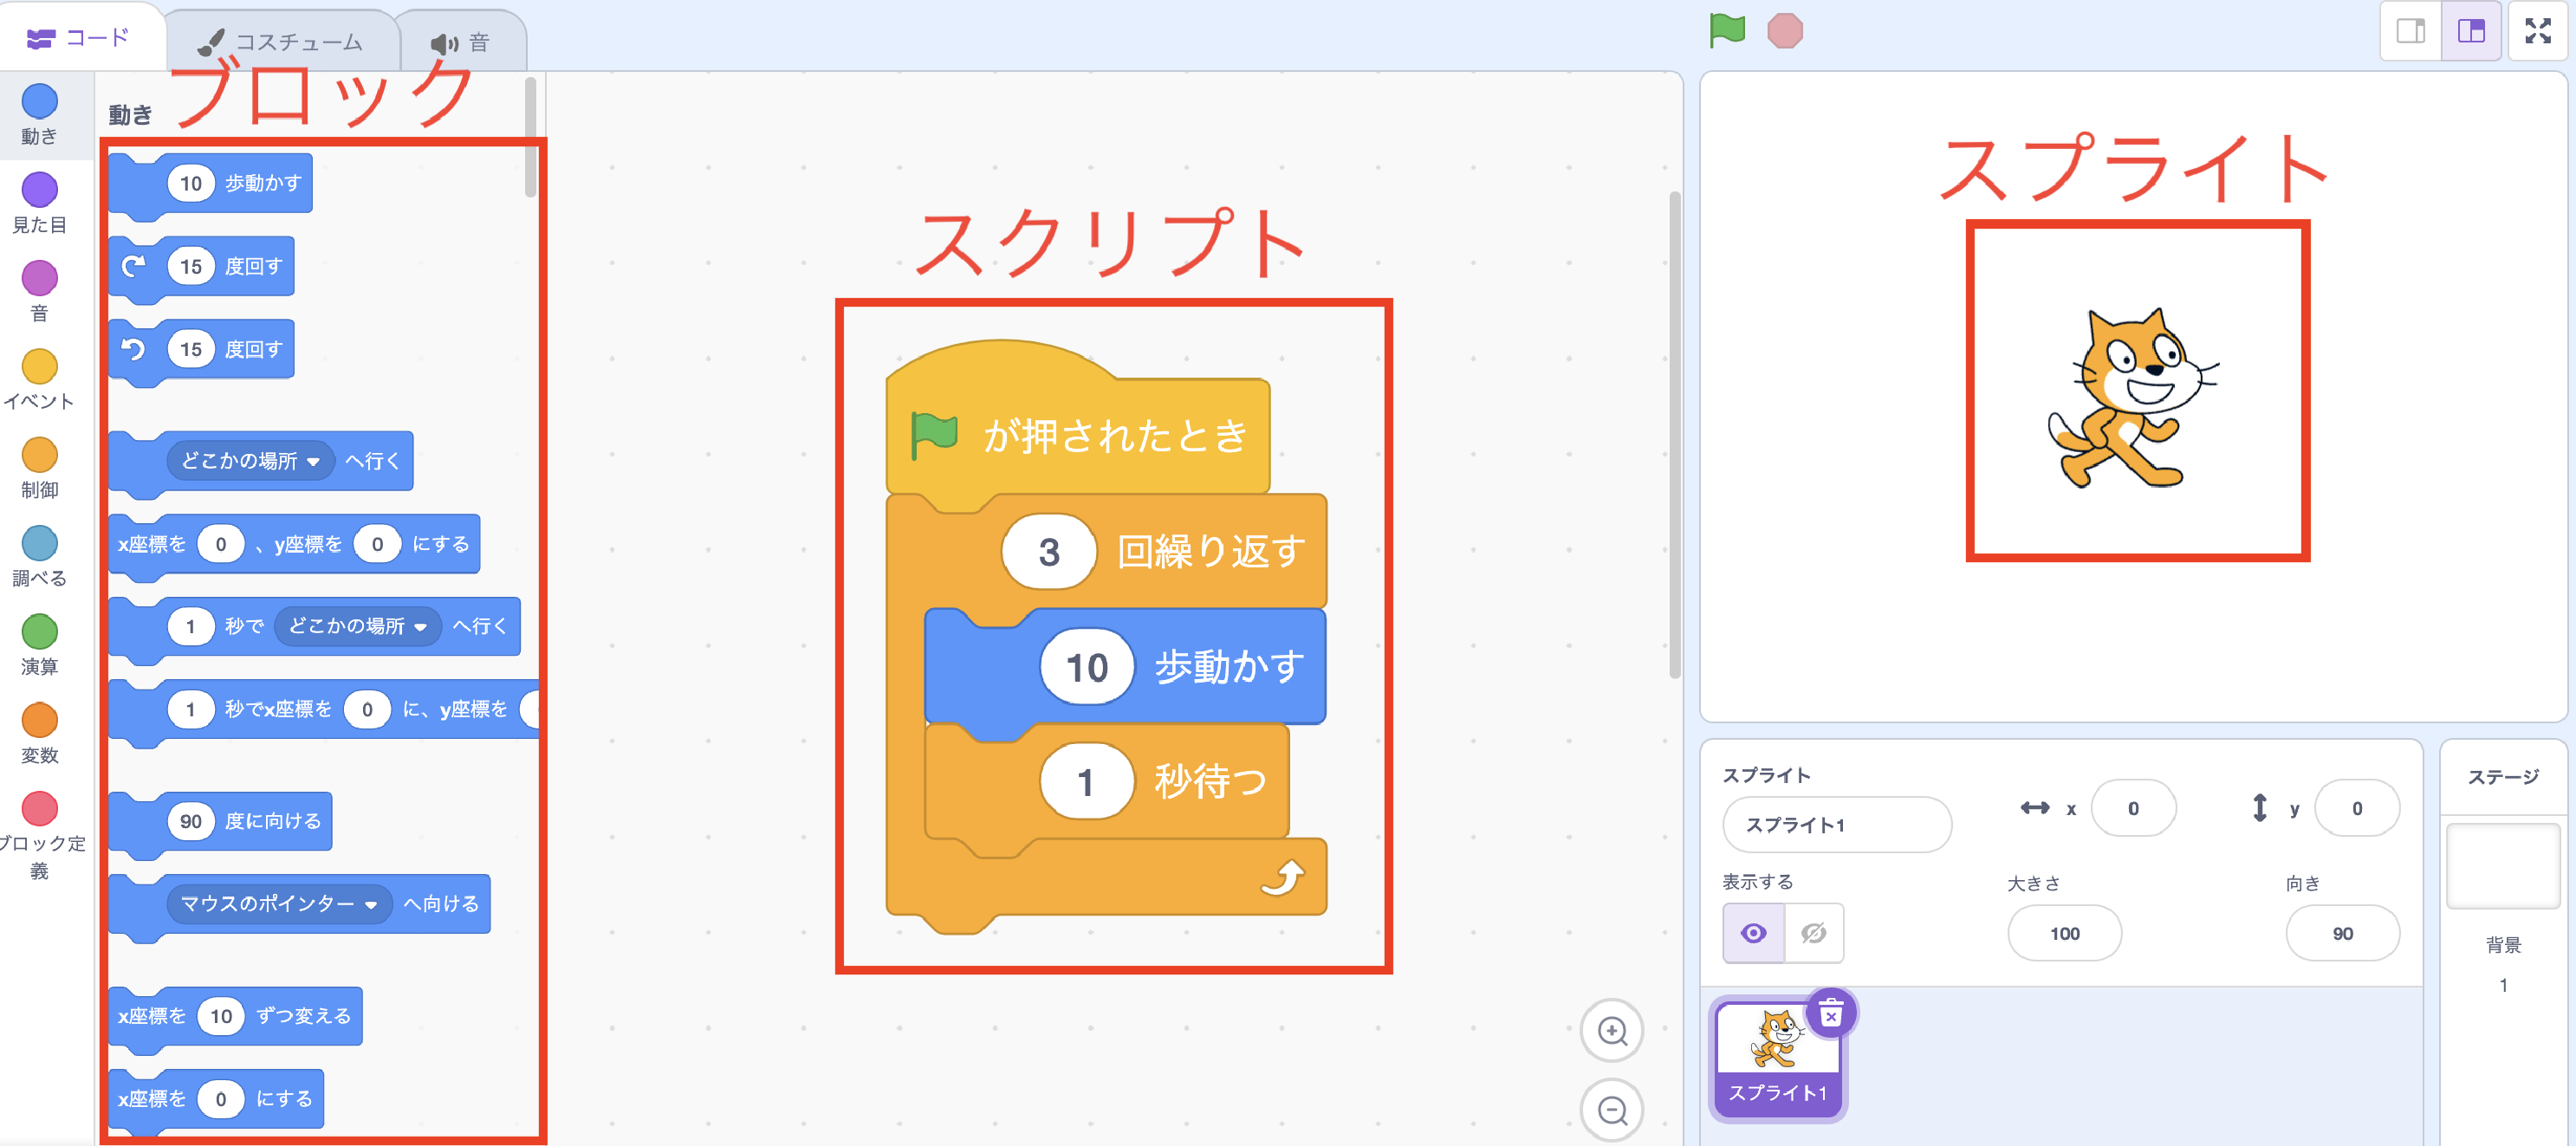
\includegraphics[width=1.0\linewidth]{Okamoto_fig/project.pdf}
	\caption{Scratchの作品制作画面}
	\label{fig:Scratch-description}
\end{figure}
%--------------------
%\subsection{従来研究:動作軌跡の類似度}
%Scratchで,ユーザはキーワード検索によって他者の作品を参照することができるが,ユーザが思い描く動作軌跡を言語化して検索することは容易でない.従来研究では,マウスを用いた描画によってユーザの動作イメージを入力することで,動作の言語化を必要としないScratch作品の直観的作品検索手法を提案している.入力と検索対象となるスプライトの動作軌跡の類似度合いを測定するために,2つの時系列データの距離を算出する動的時間伸縮法(以下,DTW)を用いており,類似動作を抽出可能な距離を明らかにした.

\subsection{従来研究: Scratchを対象とするプログラム解析}\label{subsec:analyze-scratch}

Scratchをはじめとするビジュアルプログラミング言語を用いて開発されるプログラムを調査する研究が報告されている\cite{Talbot_2020}.
%Re-Use of Programming Patterns or Problem Solving?Representation of Scratch Programs by TGraphsto supportStatic Code Analysis@WiPSCE2020
Peeratham\cite{Understanding}らは,ビジュアルプログラミングの作品に含まれるコードスメルを調査しており,プログラムで頻繁に発生する品質問題を特定し,作品を分類している.
%Understanding Recurring Quality Problems and Their Impact on Code Sharing in Block-Based Software@VLHCC2017
Peeratham\cite{techapalokul2019code}ら,およびSurisettyら\cite{Surisetty_2015}は,ビジュアルプログラミングにおけるリファクタリングツールの適用効果を調査しており,再利用されるプログラムを分類している.
また,Fein\cite{fein2022evaluation}らは,ScratchプログラムをAlonら\cite{alon2019code2vec}が提案したCode2Vecに適用して作品の分類を行い,その有用性を明らかにした.

%Code Quality Improvement for All: Automated Refactoring for Scratch@VLHCC2019
%Behavior-based clustering of visual code @VLHCC2015
これらの従来研究では,作品に使用されるブロックの種類に基づいて作品分類に取り組んでおり,それら作品が類似する動作か否かを定性的に調査している.本研究ではブロックの種類を含めたプログラムの構造の類似性にも着目し,画像オブジェクトの動作軌跡の類似性を定量的に調査する.
%プログラムの分類に取り組んでいるが,プログラム間の類似性には着目しておらず,またプログラムによって移動する画像オブジェクトの動作軌跡の類似性も確認していない.
% \todo{なぜ確認しないといけないのか?}

\subsection{従来研究:プログラムの類似度}\label{subsec:similarity of scratch}
テキストベースのプログラミング言語であるC言語やJava言語を対象としたプログラム検索手法として,特徴ベクトルに基づく手法,機械学習に基づく手法,データベースに基づく手法など,プログラムの類似性に着目する研究が報告されている\cite{Grazia_2023}.
%Luca Di Grazia and Michael Pradel. 2023. Code Search: A Survey of Techniques for Finding Code. ACM Comput. Surv. 55, 11, Article 220 (November 2023), 31 pages. https://doi.org/10.1145/3565971

Scratchでは,スプライトの動作軌跡が類似していても実装方法が異なることがある.一方で,プログラムは類似していてもスプライトの動作が異なることもある\cite{Surisetty_2015}.前者は,同じ機能を実装するための多様な方法があることが示唆されるが,後者はScratchにおけるプログラミング検索においてユーザが期待する作品の収集の妨げになることが示唆される.
%このことから,Scratch上ではプログラムが類似していても,一概に似ている作品であるとは言えず,プログラムの出力結果であるスプライトの動作軌跡も考慮する必要がある.

%Scratchで,ユーザは類似するプログラムが混在する膨大な検索結果の中から,多様なプログラムの実装方法を含む作品を探すことは手間がかかり容易でない.従来研究では,Scratch作品において類似したプログラムの実装方法を持つ作品を各々紐づけるために,類似プログラムを判定するための手法を提案した.具体的には,Scratchプログラムを抽象構文木(以下,AST)として捉え,プログラム間の編集距離をプログラムの類似度として算出しており,類似プログラムを判定するための基準を明らかにした.


\subsection{動機}\label{subsec:reason}

本研究では,Scratchにおいて制作されるプログラムの類似度の測定手法,およびオブジェクト動作軌跡の類似度の測定手法を提案し,図\ref{fig:sample-scatter}に示すように,プログラムが類似するか否か,オブジェクト動作軌跡が類似するか否かの4種類に分類することで,プログラムの類似性とオブジェクト動作軌跡の類似性の乖離を明らかにする.特に,図中の(2)に示すような第2象限(プログラムは類似するが,オブジェクト動作軌跡が類似していない),図中の(4)に示すような第4象限(オブジェクト動作軌跡は類似するが,プログラムは類似していない)のような,プログラムの類似度とオブジェクト動作軌跡類似度が乖離する作品を分析する.

図\ref{fig:pattern1}は,第2象限に含まれる作品対の事例を示す.図\ref{fig:pattern1}中の(1),(2)のプログラムではともに同じ種類のブロックを用いて実装しているが,(1)の作品ではオブジェクトが矩形に移動し,(2)の作品ではオブジェクトが円形に移動するため,動作軌跡は異なる.(1)(2)ではそれぞれの回転角度が90度,15度であるため,プログラムは類似するが,動作軌跡が異なる作品となる.
%これは,角度を変えるブロックの数値の差がオブジェクトの動作軌跡に影響したことが原因である.このように,ブロック内の数値が異なると,プログラムが類似しても動作軌跡が類似しないことが示唆される.

図\ref{fig:pattern2-1}と図\ref{fig:pattern2-2}は,第4象限に含まれる作品対の事例を示す.

図\ref{fig:pattern2-1}中の(1),(2)のプログラムはともにオブジェクトが右に移動する同じ動作軌跡を描くが,プログラムに使用されるブロックは大きく異なる.Scratchでは座標の移動に関わるブロック以外にも,(2)で使用している見た目を変更するブロックや音を鳴らすブロックのように移動には直接関係のないブロックを含むこともある.そのため,座標ブロック以外のブロックが作品内に多く存在すると,動作軌跡が類似してもプログラムが類似しないことがある.

また,図\ref{fig:pattern2-2}も(1),(2)のプログラムは同じ動作軌跡を描くが,異なるブロックを使用する,プログラムが類似していない作品である.この作品では,(1)ではループを用いて実装,(2)ではループを用いずに,順次にブロックを連ねて実装しており,動作軌跡は類似するが,プログラムが異なる作品となる.

%--------------------
\begin{figure}[t]
	\centering
	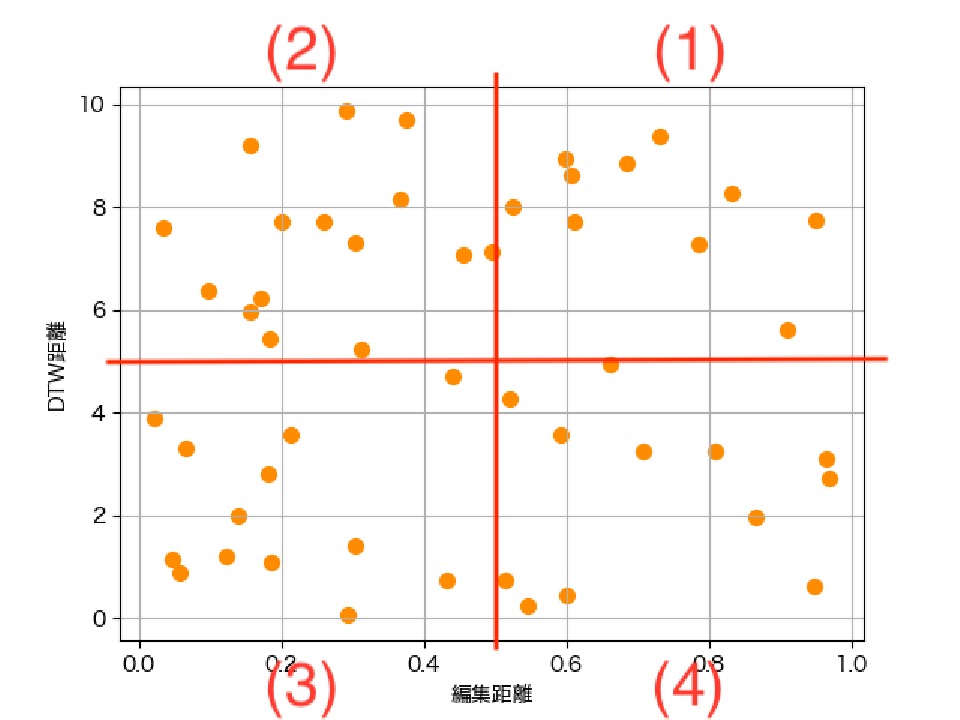
\includegraphics[width=1.0\linewidth]{Okamoto_fig/out-sample.pdf}
	\caption{プログラムの類似度と動作軌跡の類似度の関係性を示した散布図の例}
	\label{fig:sample-scatter}
\end{figure}
%--------------------
\begin{figure}[t]
	\centering
	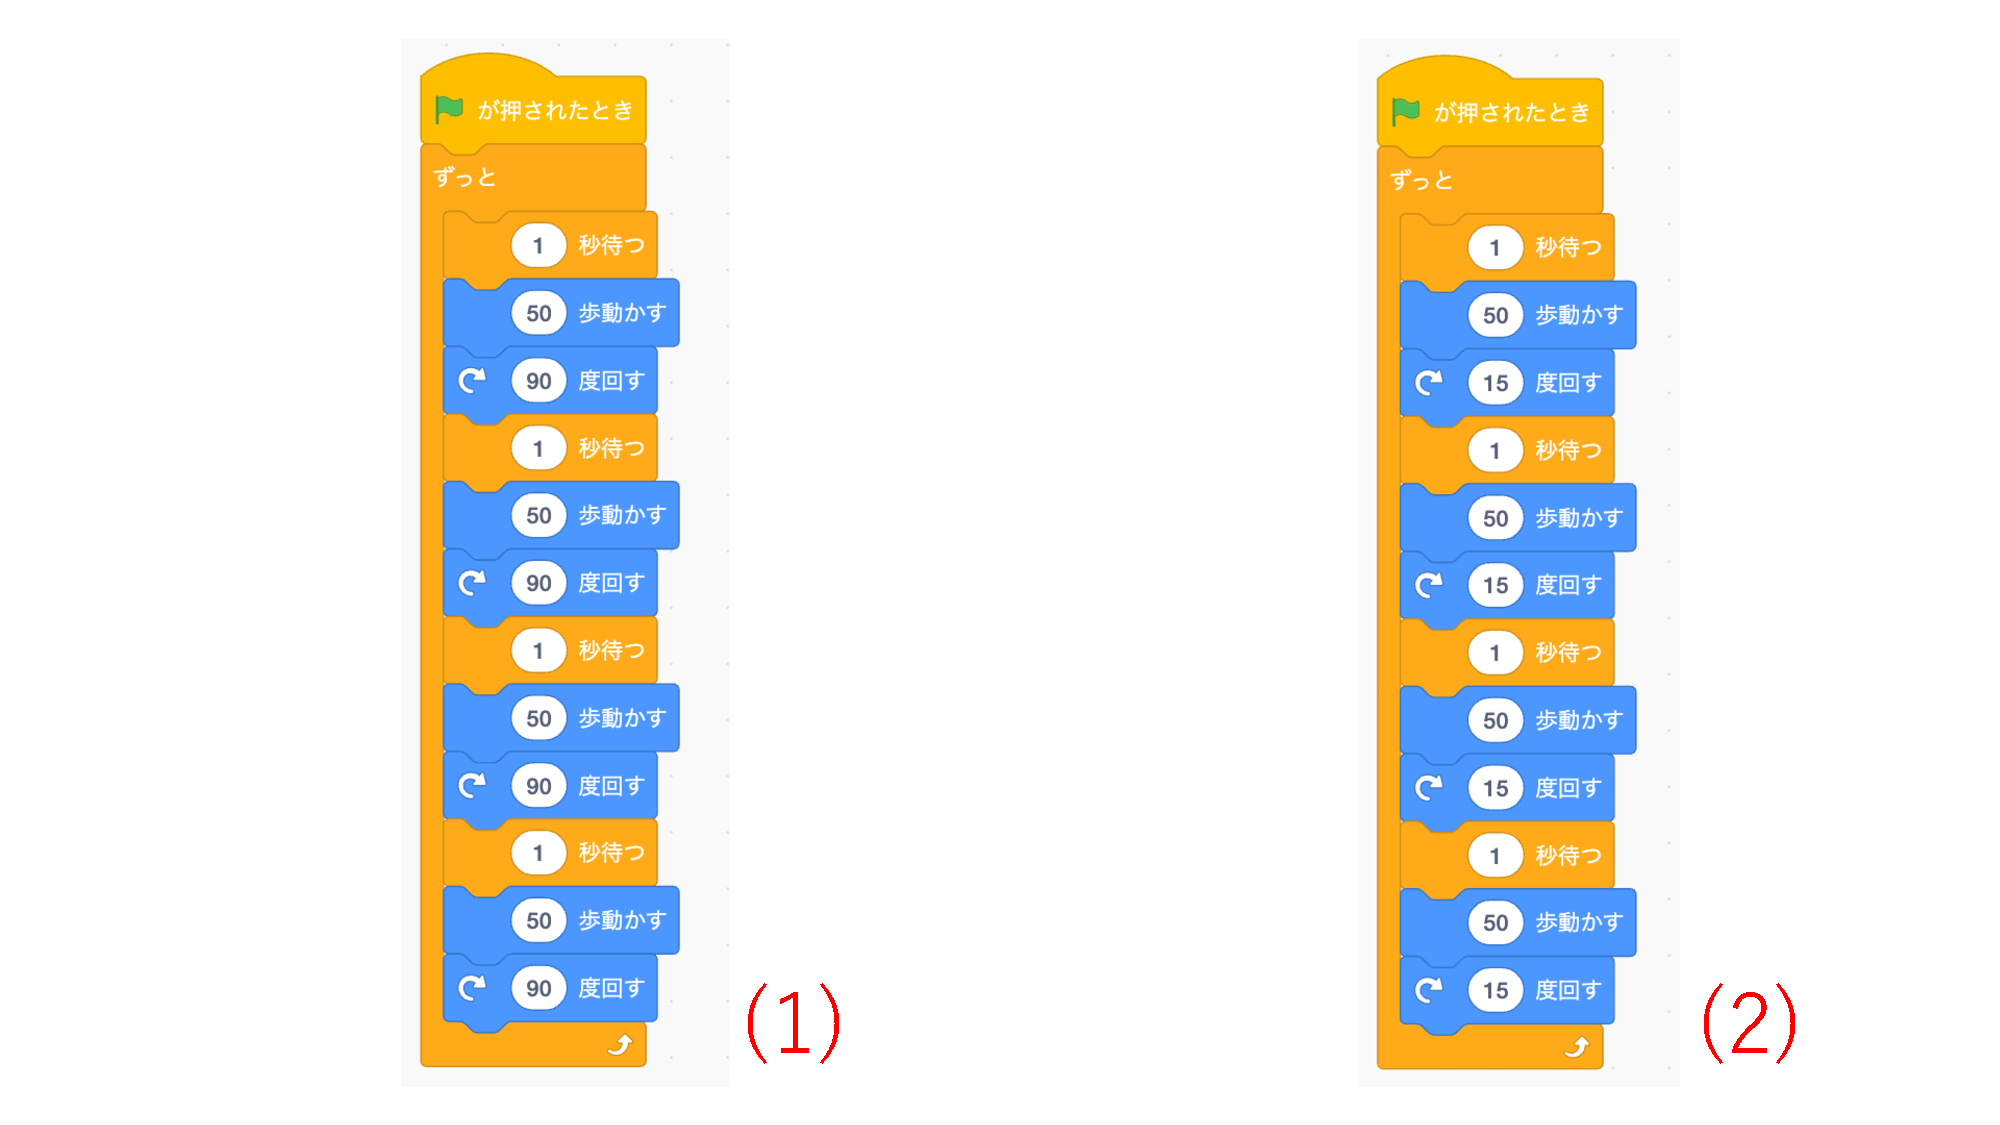
\includegraphics[width=1.0\linewidth]{Okamoto_fig/pattern1.pdf}
	\caption{プログラムは類似するが,オブジェクト動作軌跡が類似していない作品の例}
	\label{fig:pattern1}
\end{figure}
\begin{figure}[t]
	\centering
	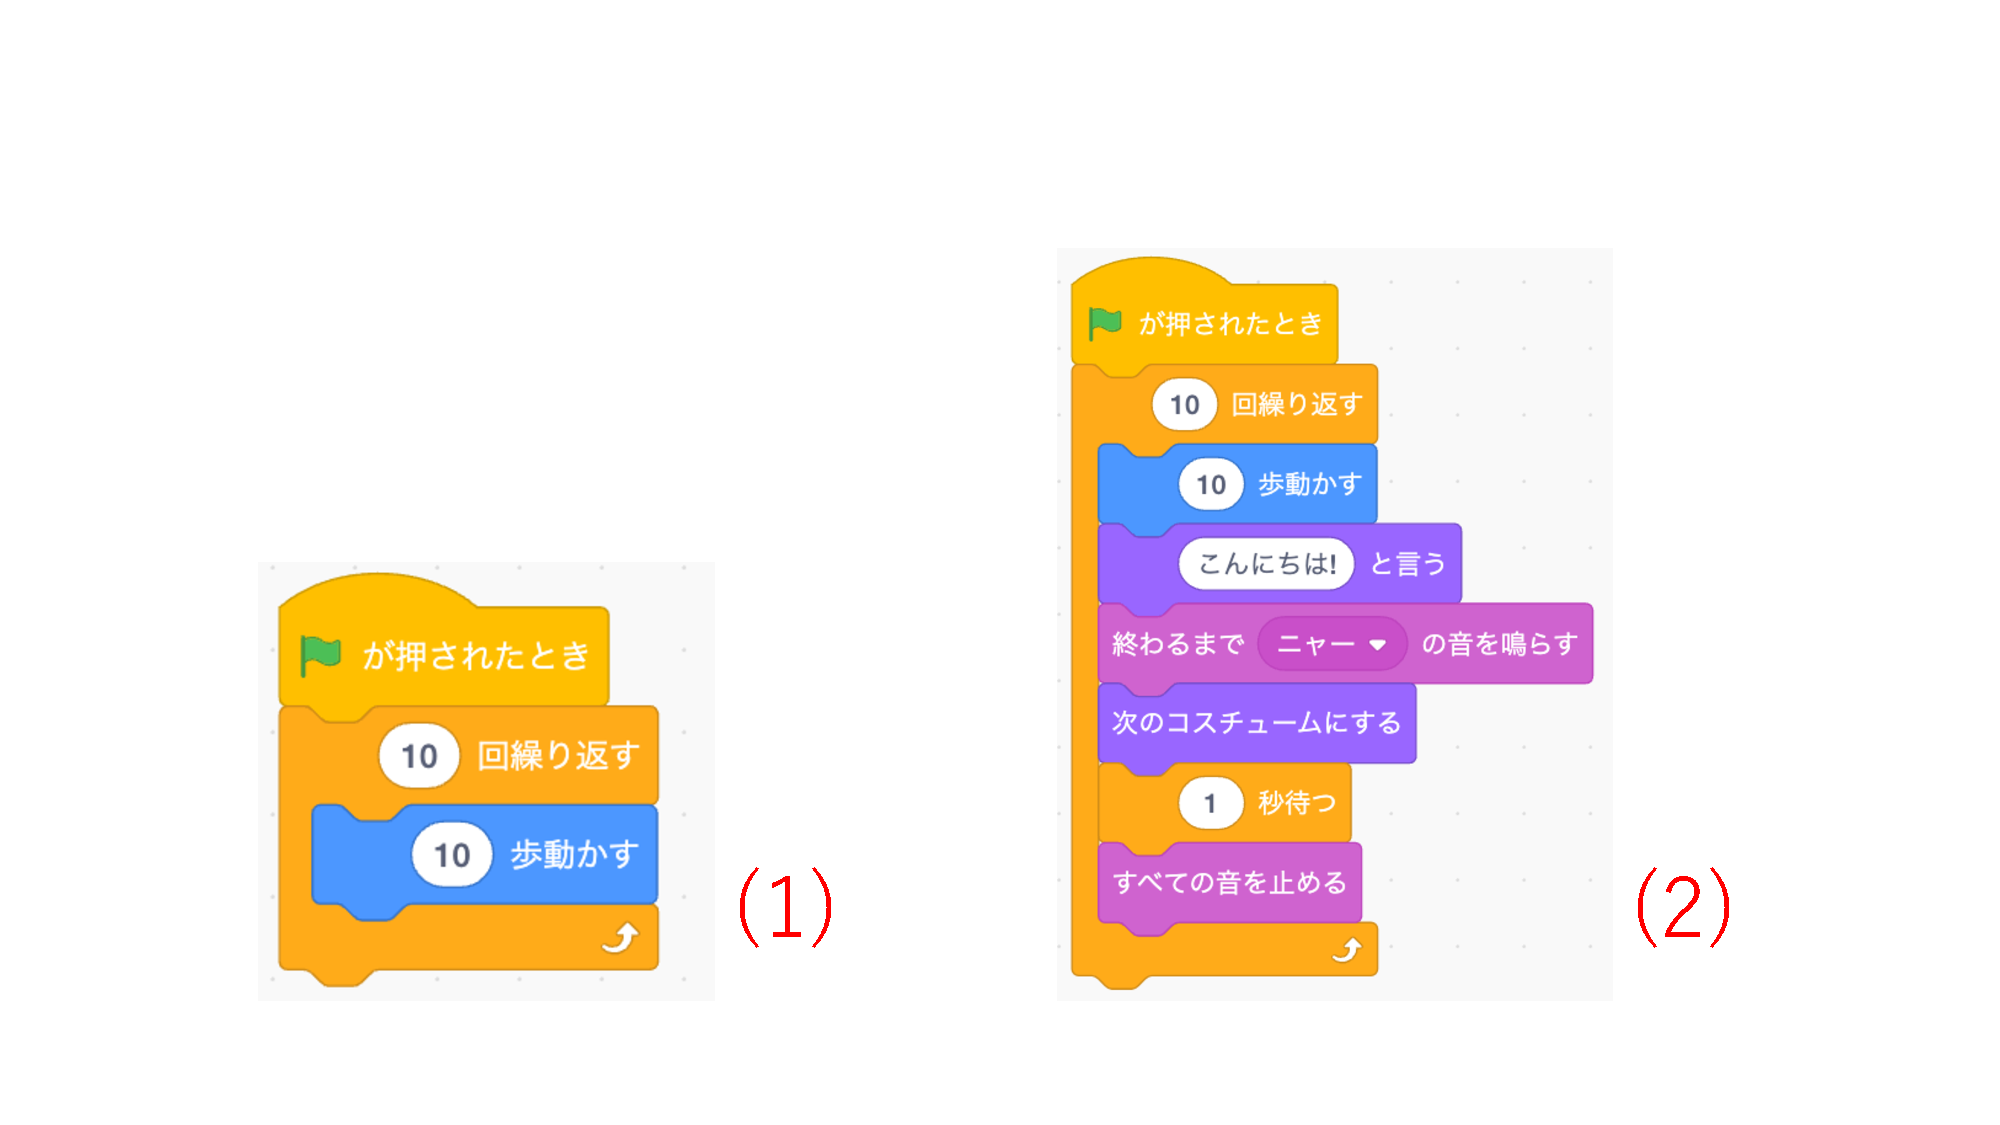
\includegraphics[width=1.0\linewidth]{Okamoto_fig/pattern2-1.pdf}
	\caption{オブジェクト動作軌跡は類似するが,プログラムが類似していない作品の例1}
   \vspace{-2mm}
	\label{fig:pattern2-1}
\end{figure}

\begin{figure}[t]
	\centering
	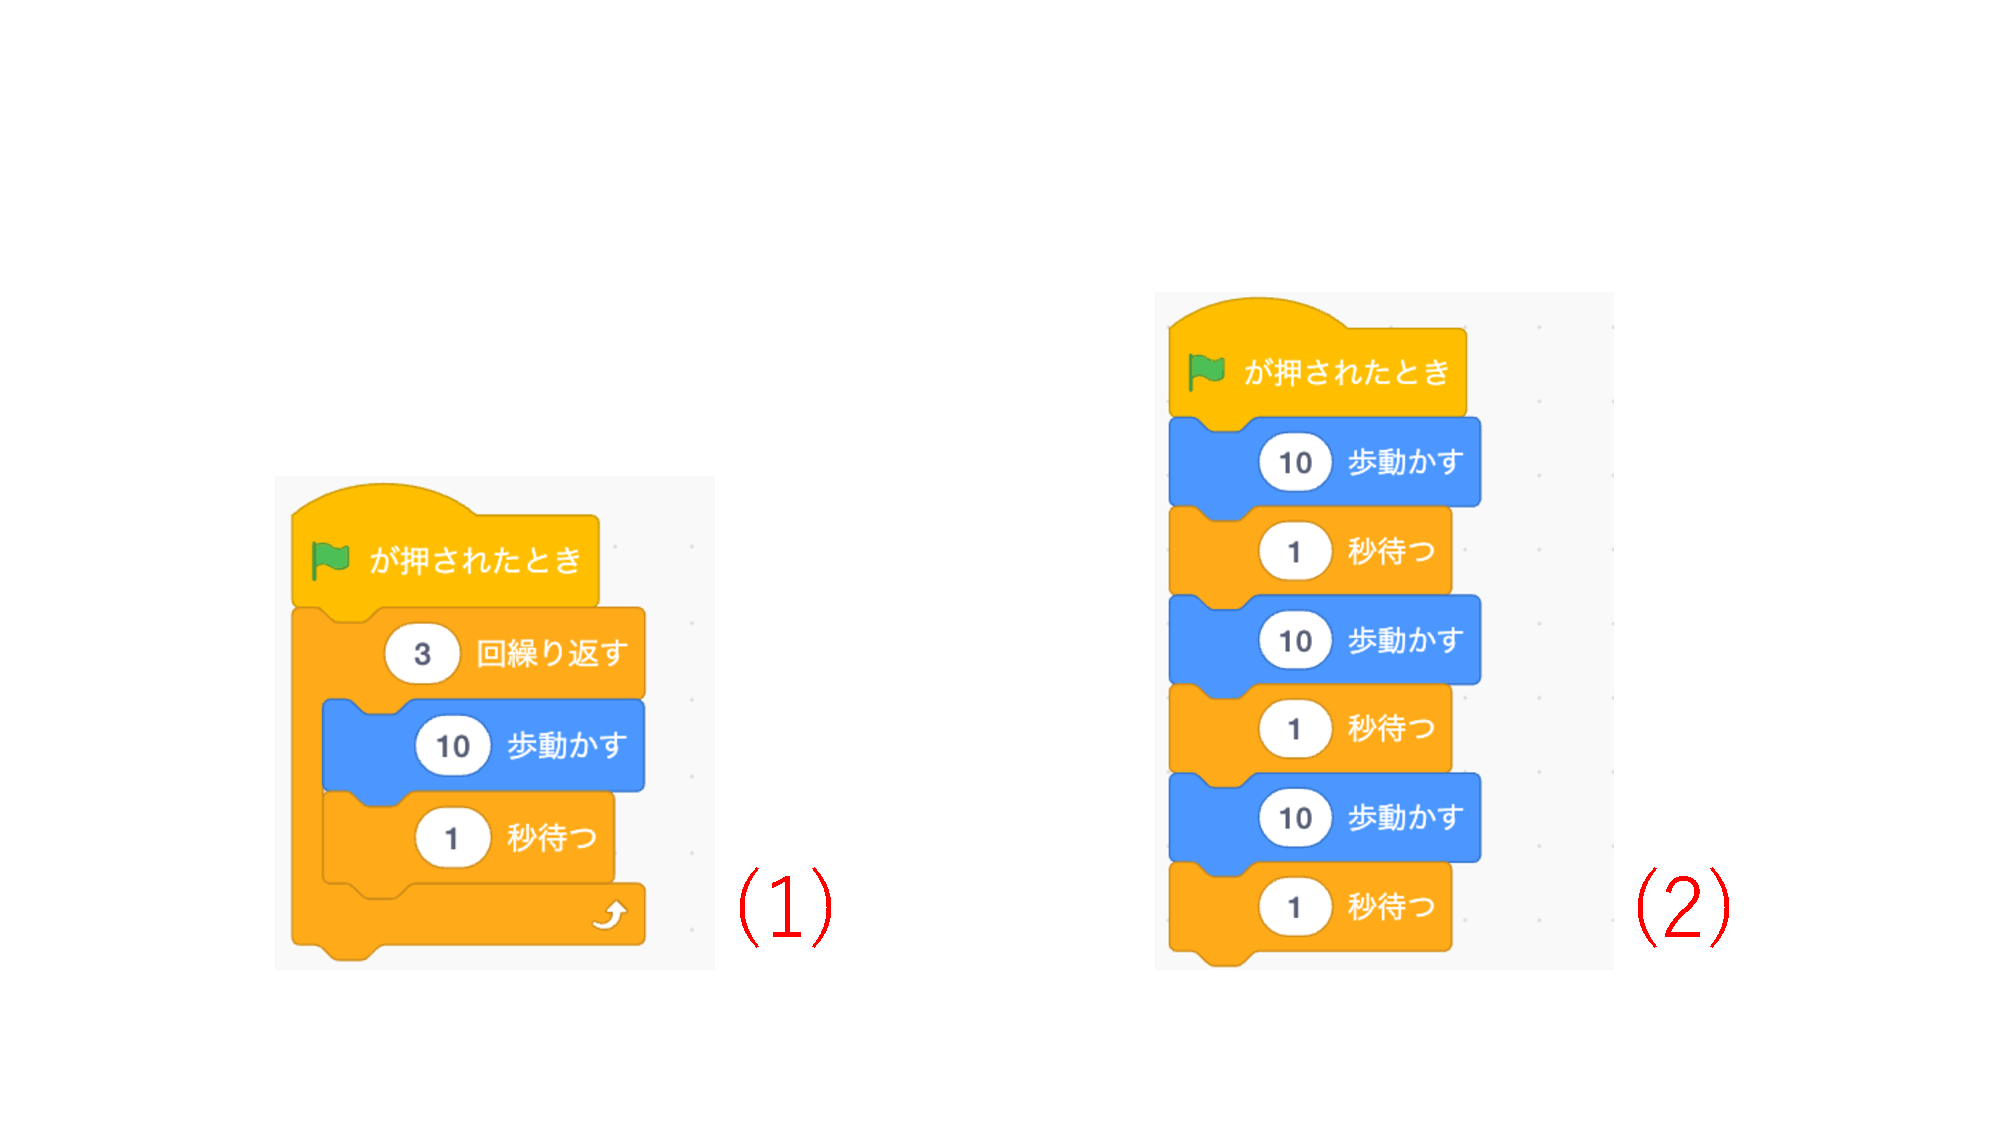
\includegraphics[width=1.0\linewidth]{Okamoto_fig/pattern2-2.pdf}
	\caption{オブジェクト動作軌跡は類似するが,プログラムが類似していない作品の例2}
   \vspace{-2mm}
	\label{fig:pattern2-2}
\end{figure}


% \begin{itembox}[l]{Research Question}
% 同作品間における動作軌跡の類似度とプログラムの類似度に相関はあるか
% \end{itembox}

%%%%%%%%%%%%%%%%%%%%%%
\section{類似度の測定手法}\label{sec:Similarity}
%%%%%%%%%%%%%%%%%%%%%%

本章では,スプライトの動作軌跡の類似度,およびプログラムの類似度の算出方法について述べる.

\subsection{動作軌跡の類似度測定手法}\label{subsec:Similarity movement measurement}

作品に含まれるスプライトの動作軌跡の類似度を算出するために,本研究ではスプライトの座標の動作軌跡を追跡し,異なる作品に含まれるそれぞれのスプライトの動作軌跡の類似度を動的時間伸縮法(DTW: Dynamic time warping)を用いて算出する.著者らは,先行研究\cite{Fukuchi2021}において動作軌跡の類似度の測定手法を開発しており,2つの手順(1. スプライトを配置する座標の時系列データの取得,2. 2作品間のスプライトの動作軌跡の類似度を算出)により類似度を算出する.

\subsubsection{スプライトを配置する座標の時系列データの取得}

先行研究\cite{Fukuchi2021}では,異なる作品に含まれるスプライトの動作軌跡を追跡するために,Scratchの作品中の実行画面内でスプライト画像の移動をLoweらが提案したSIFT(Scale-Invariant Feature Transform)\cite{lowe1999object}を用いて画像中の特徴点を抽出し,スプライトの座標変化を取得していた.しかし,当該手法は事前に追跡対象とするスプライト画像を決定するため,Scratchが提供する画像のみが対象となり,分析対象とする作品数が限られてしまう.また,実行画面の動画を事前に取得する必要があり,データ収集に膨大な時間を要することが課題であった.これらの課題解決として,本研究ではScratch APIにより取得できる作品で使用されるブロック情報に基づき,次の手順でスプライトの座標を追跡する.
\begin{enumerate}
    \item Scratchが公開しているAPIを用いて作品情報を含むJSONファイルを取得し,複数スプライトがある場合は先頭に存在するスプライトのスクリプト,ブロック情報を抽出
    \item ブロックを実行順序順にソートして,座標変化を含むブロックから座標情報を抽出
    \item 初期座標と2.で抽出した座標情報のデータから座標変化を算出し,時系列順に出力
    \item ループは一度のみの実行とし,入力操作を含む作品も入力後の座標変化も含めて算出
\end{enumerate}

\subsubsection{DTWを用いて座標同士の距離を算出}

従来研究では,スプライト間の動作軌跡として座標変化の類似度を算出において,動的時間伸縮法(DTW: Dynamic time warping)を用いて算出する.DTWは2つの時系列データの距離を動的計画法に基づいて算出する手法である.DTWでは,2つの時系列データの各点の距離を総当たりで全て求め,2つの時系列データの累積距離が最短となる経路であるDTW距離を算出する.図\ref{fig:dtw}は,DTWの概略図を示す.DTWでは,距離を算出する2つの時系列データS=$s_{1}$,$s_{2}$,$s_{3}$,…$s_{15}$, T=$t_{1}$,$t_{2}$,$t_{3}$,…$t_{10}$をそれぞれ縦軸,横軸に並べ,各マス(i,j)における要素$s_{i}$と$s_{j}$間の距離を算出する.図\ref{fig:dtw}中では,マスの色が薄いほど距離が近く,色が濃いほど距離が遠いことを指す.時系列データSとTの各要素の累積距離が最も短くなる経路を探し出し,その累積距離を2つの時系列データのDTW距離として算出する.DTW距離の値が小さいほど,動作軌跡の類似度は大きいと言える.
%--------------------
\begin{figure}[t]
	\centering
	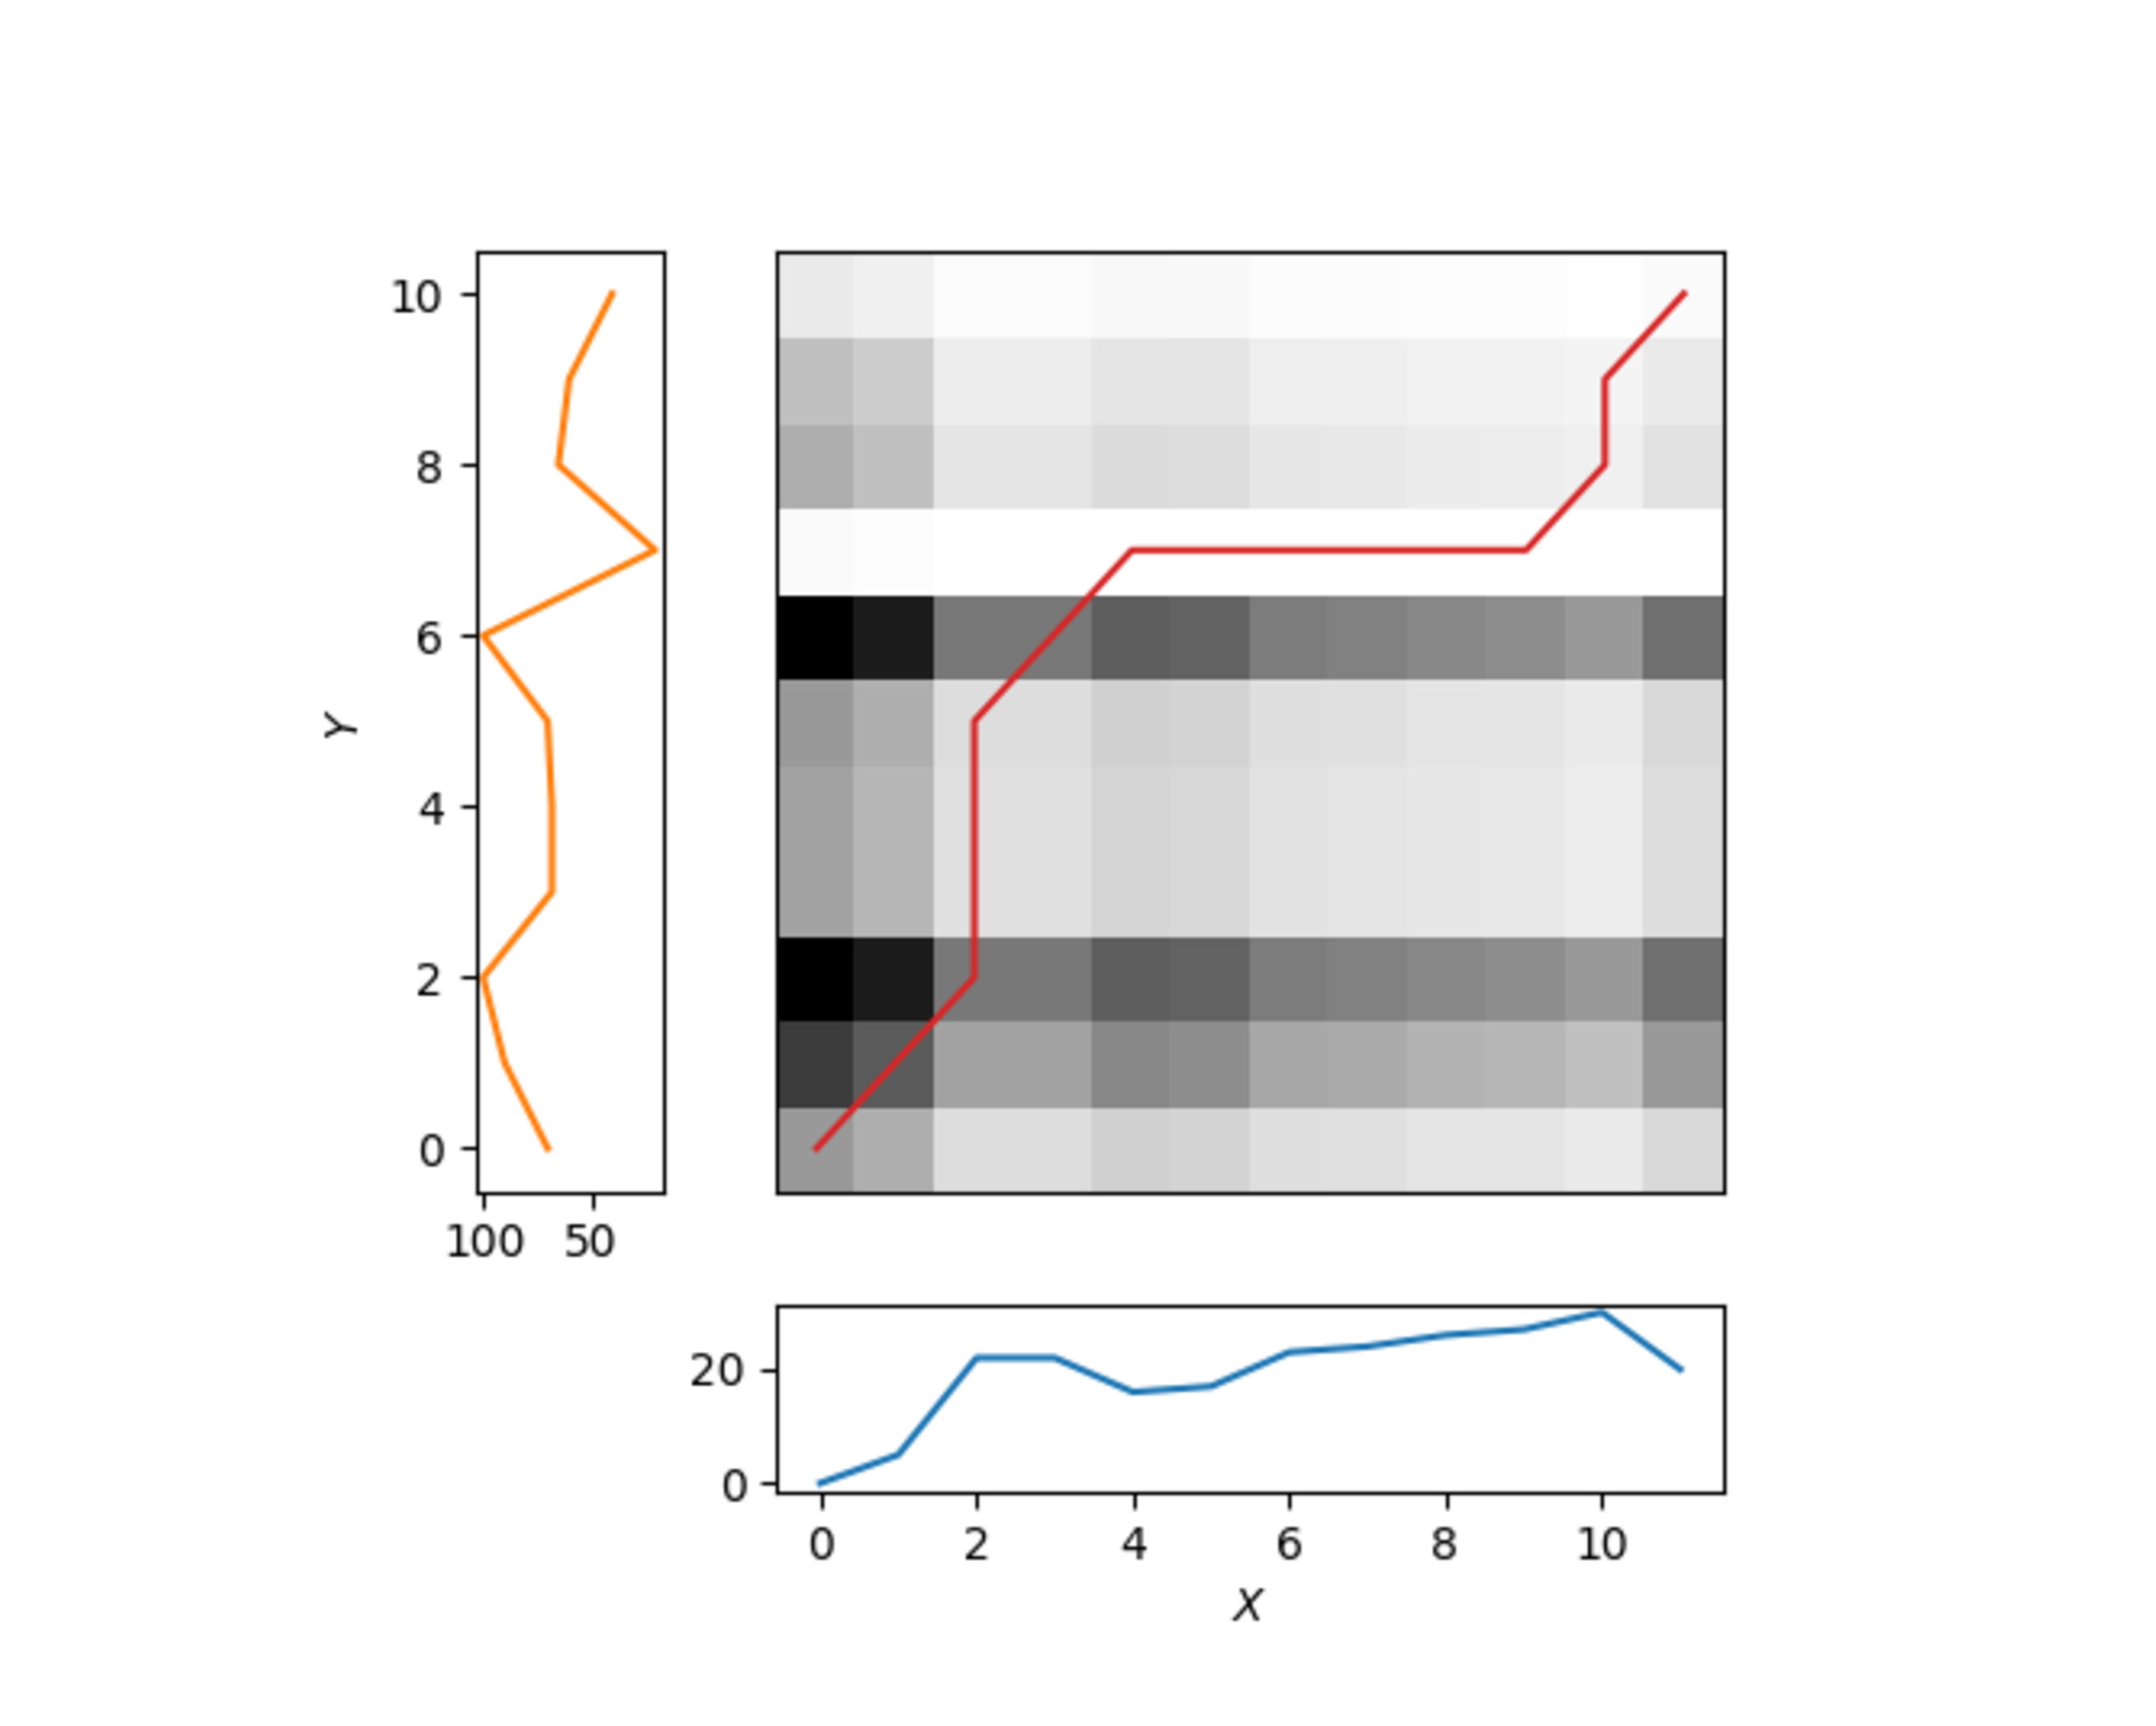
\includegraphics[width=1.0\linewidth]{Okamoto_fig/dtw-example.pdf}
	\caption{動的時間伸縮法(DTW)の概略図}
	\label{fig:dtw}
\end{figure}
%--------------------

DTW距離では,図\ref{fig:coordinate}の作品Aと作品Bのように座標が離れている場合でも,座標にかかわらず移動軌跡が類似していれば類似動作として抽出している.従って,3.1.1で出力した時系列データを最小値0,最大値1の時系列データに正規化している.
%------------------------
\begin{figure}[t]
	\centering
	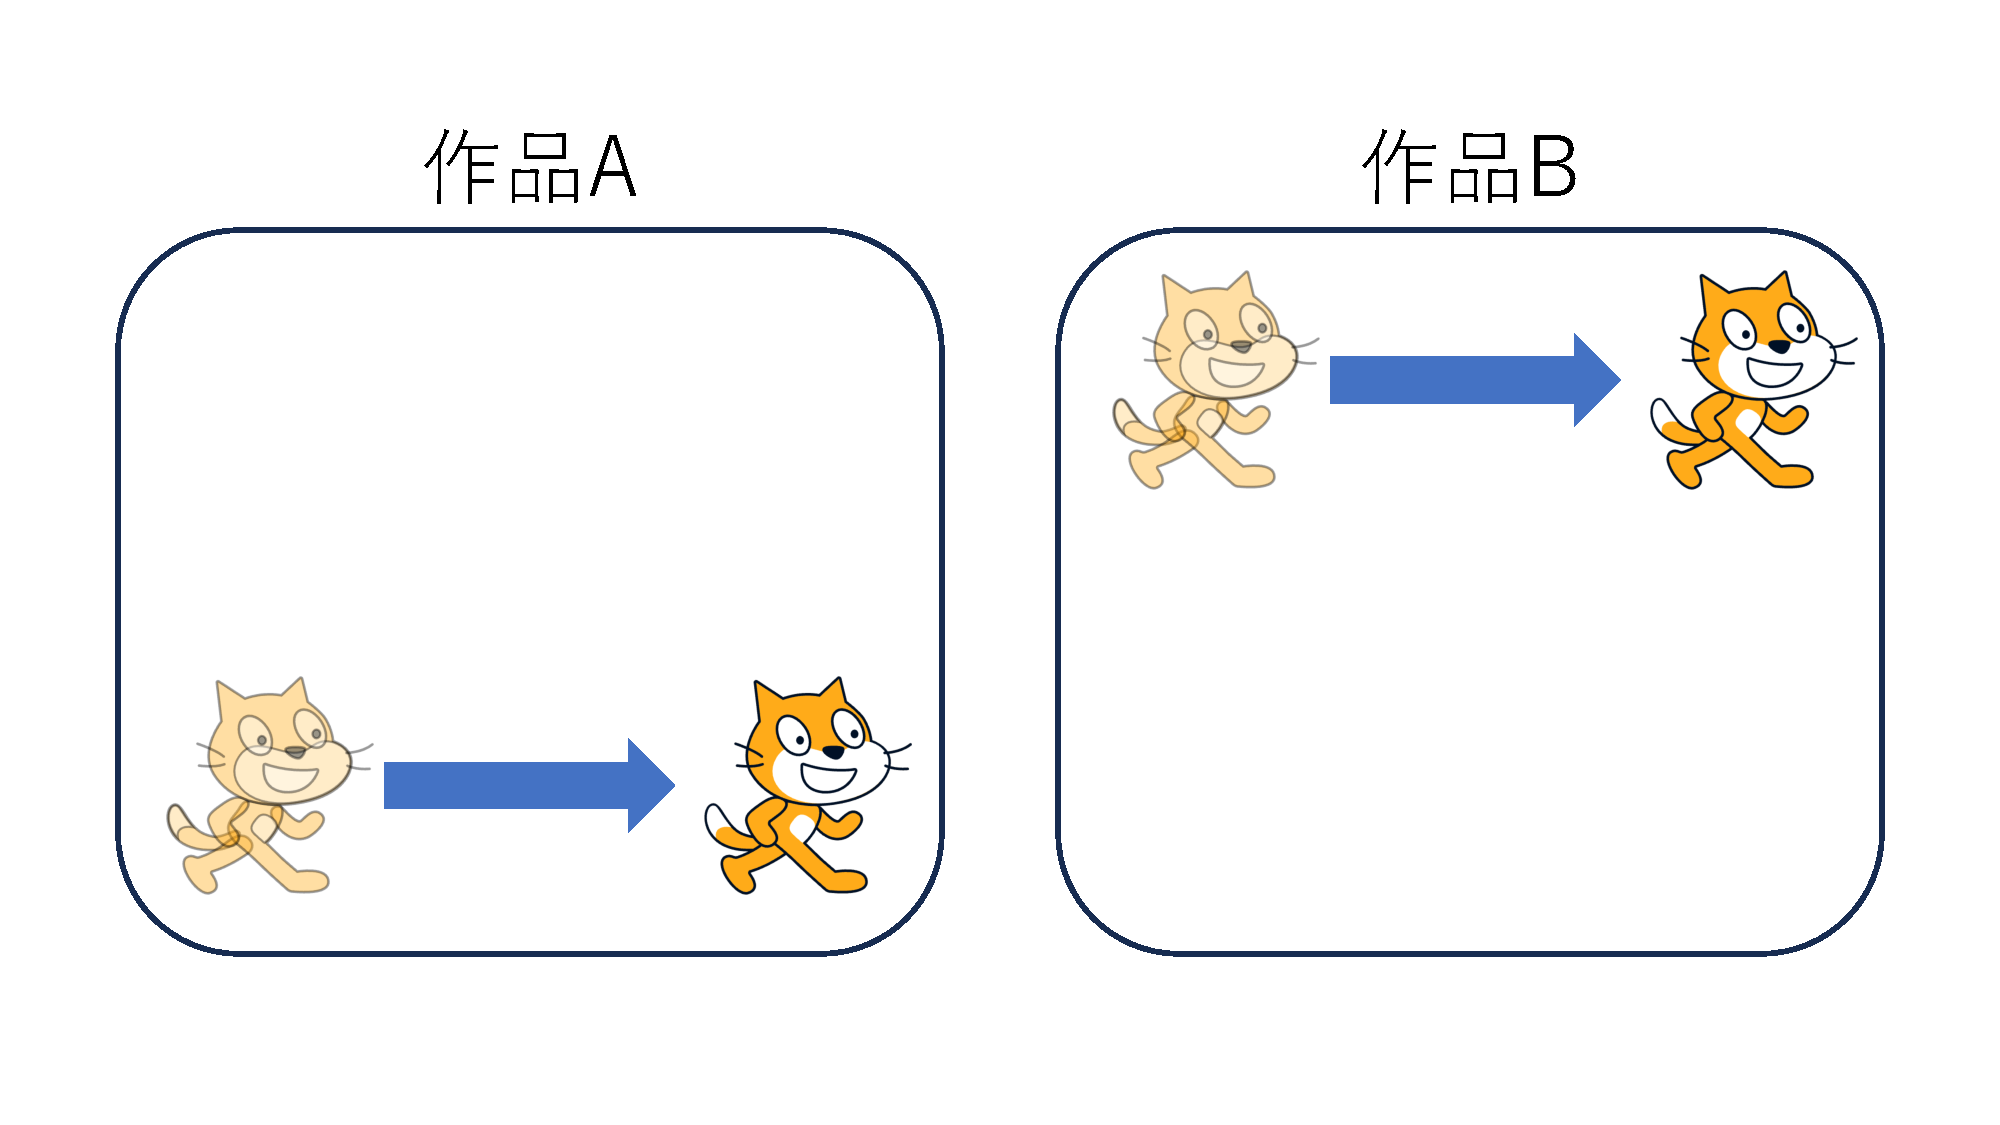
\includegraphics[width=1.0\linewidth]{Okamoto_fig/coordinate.pdf}
 \vspace{-5mm}
	\caption{座標が離れていて軌道が類似している作品例}
	\label{fig:coordinate}
\end{figure}
%------------------------

\subsection{プログラムの類似度測定手法}\label{subsec:Similarity program measurement}

2.3節で述べた通り,テキストによるプログラム類似度の測定手法は多数提案されている.本研究では,Scratchで作成されるプログラムから抽象構文木を生成し,抽象構文木間の編集距離を用いてプログラム類似度を算出する.

\subsubsection{Scratchプログラムから抽象構文木への変換}

抽象構文木は,プログラムから言語の意味に関係のない情報を取り除き,意味に関係のある情報のみを取り出し,抽象化した木構造のデータである.

本研究では,Scratchが公開しているAPIを用いて取得できる作品に使用されるブロックに基づき,作品のスクリプト情報を抽象構文木に変換する.図\ref{fig:abst}は,Scratch作品のスクリプトを抽象構文木に変換したときのイメージを示す.図\ref{fig:abst}の(1)に示すScratchプログラムを抽象構文木に変換すると,(2)となる.本研究で扱う抽象構文木では,(2)のようにな木構造を出力する.ブロック名をノードのラベルとし,1つのスクリプトにおけるすべてのブロックのつながりを示す.スクリプトは(2)に示す「SCRIPT」を木の頂点とし,スクリプトの実行順序に従ってブロック名を左から1つの階層にノードラベルとして連ねる.制御ブロックをはじめとした,ブロックを内包する入れ子構造のブロックは,(2)に示した「gotoxy」,「turn」のように階層を1つ深くして表現する.また,本研究ではプログラム構造のみに着目して類似度を算出するため,制御ブロックが含む引数やその他の演算子等は考慮しない.
%----------------------
\begin{figure}[t]
	\centering
	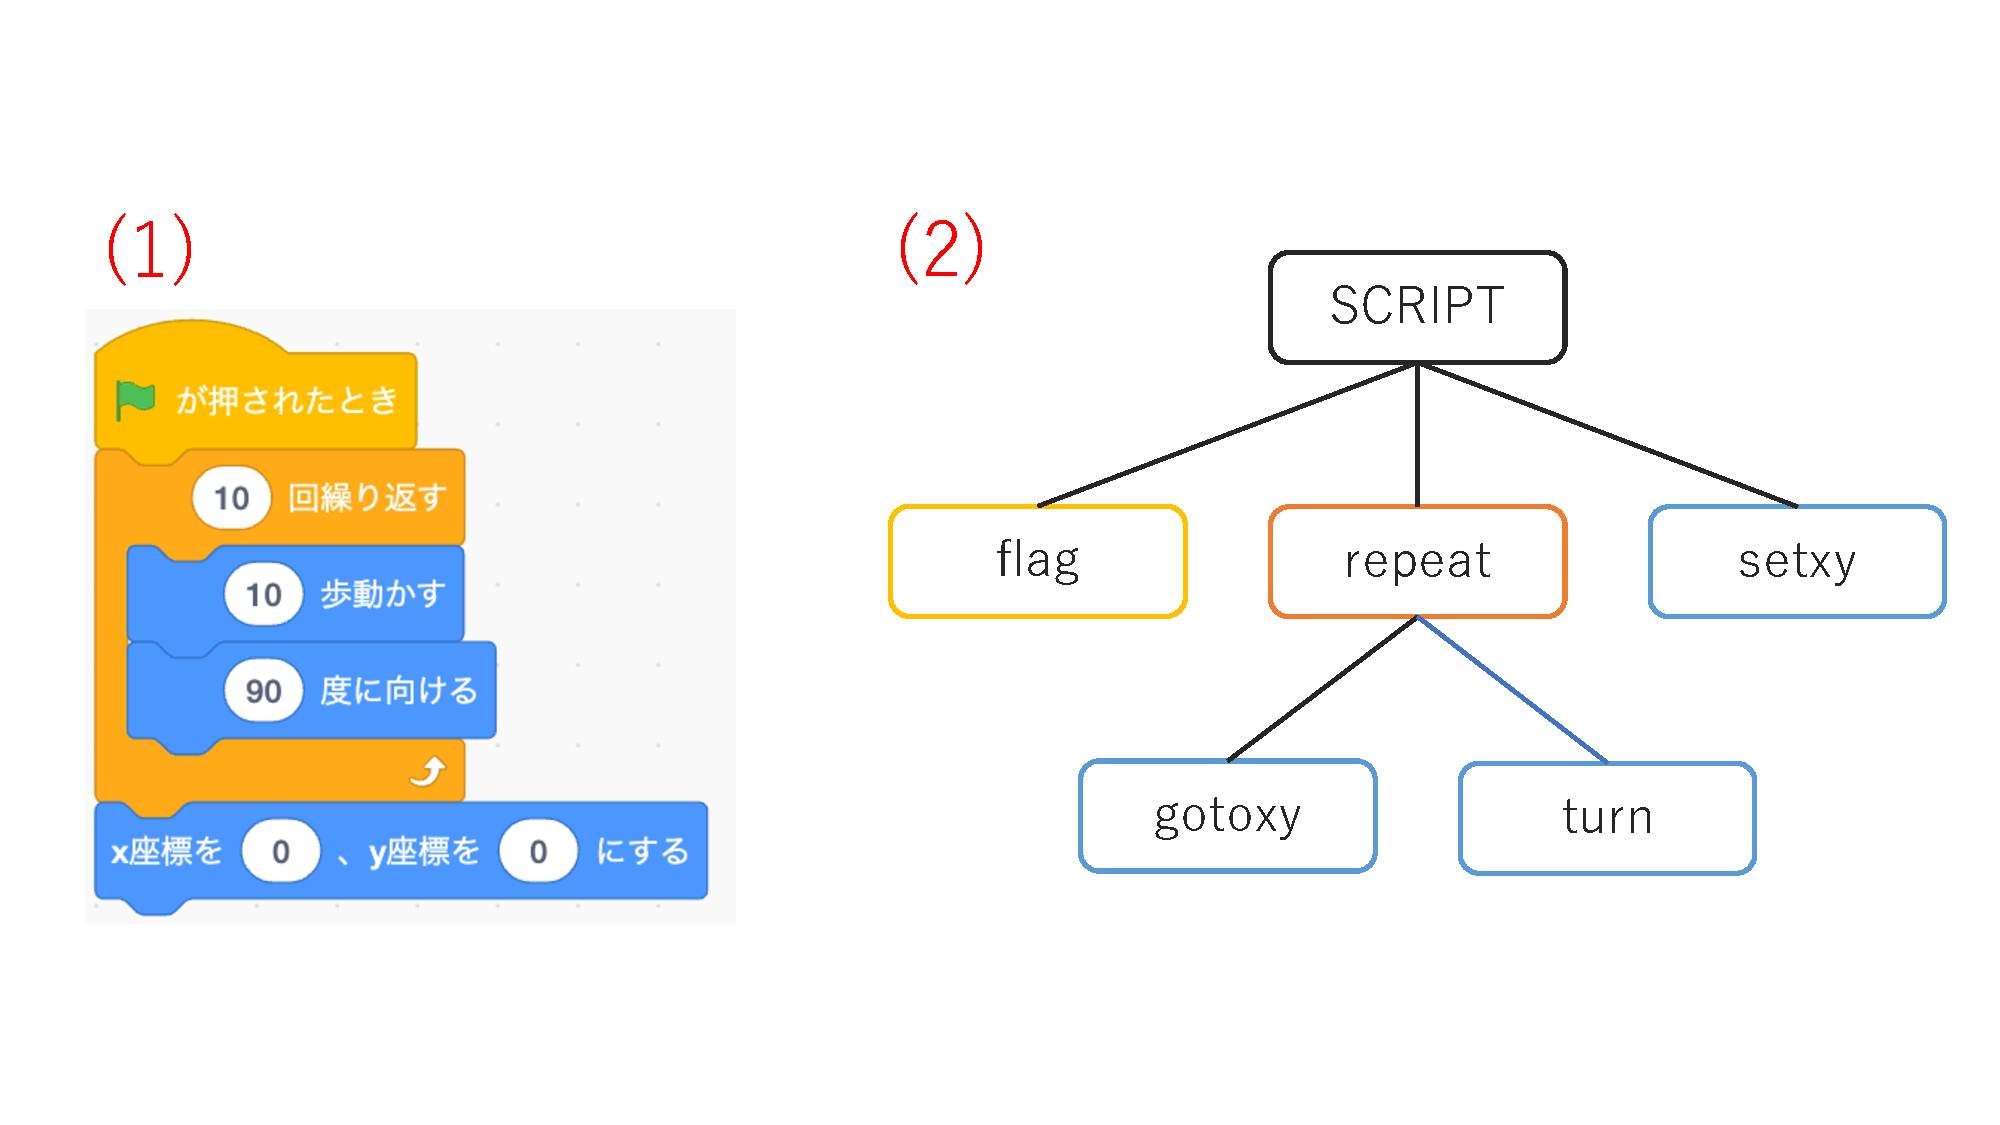
\includegraphics[width=1.0\linewidth]{Okamoto_fig/abst.pdf}
	\caption{Scratchプログラムから抽象構文木化}
	\label{fig:abst}
\end{figure}
%----------------------
%参考になりそう.https://sdl.ist.osaka-u.ac.jp/pman/pman3.cgi?DOWNLOAD=569


\subsubsection{編集距離によるプログラム類似度の算出}
本手法では,異なる作品のスクリプトから変換した抽象構文木に基づき,抽象構文木間の編集距離を算出する.抽象構文木における編集距離は,片方の抽象構文木をもう片方の抽象構文木と等しくするために行う最小の編集回数である.編集の定義は,ノードの挿入,ノードの削除,ノードラベルの置換の3種類であり,編集回数とはそれぞれを行った回数の合計数のことである.また,編集距離はブロックの長さに大きく影響を受けるため,算出した編集距離を作品対におけるスクリプト規模の大きい作品のブロック長で除算することで最小値0,最大値1に正規化した値を編集距離とする.編集距離が小さいほど,プログラムの類似度は大きいことを示す.

%%%%%%%%%%%%%%%%%%%%%%
\section{動作軌跡類似度とプログラム類似度の関係性分析}\label{sec:Analysis}
%%%%%%%%%%%%%%%%%%%%%%

\subsection{データセット}
Scratchは,バージョン3.0のリリースにおいて大幅なブロックの追加や仕様が変更された.本研究では,共通の学習環境で制作された作品を比較するために,バージョン3.0がリリースされた2019年1月3日以降に制作された作品を対象とする.また,動作軌跡の計算を複雑化せず,ある程度のプログラム規模を有する作品を対象とするために,次の条件によって分析対象とする4000件の作品を時系列順に収集した.
\begin{itemize}
    \item 並列に同じ種類のイベントブロックが存在しない
    \item 独自に定義するブロック,メッセージブロックが存在しない
    \item ブロック数が5つ以上
\end{itemize}

\subsection{アプローチ}\label{subsec:approach}

データセットとして収集した4,000件の作品を対象に,\ref{sec:Similarity}章で述べた動作軌跡類似度,プログラム類似度を総当たりで測定し,作品のプログラムが類似するか否か,スプライト動作軌跡が類似するか否かの4種類に分類する.また,プログラムと動作軌跡がそれぞれ類似しているか否かは,先行研究で示された閾値に基づいて判断する.

\noindent\textbf{[プログラム類似度の閾値] }先行研究\cite{Mikura2022}では,編集距離を用いた類似スクリプトの紐付けを行った結果,閾値を0.50にしたときに最も分類の精度が高くなった.しかし,データセット量が少なかったことから,その閾値の妥当性は示されていない.,本研究では編集距離0.50以下をプログラムが類似する境界値とし,本研究における閾値の妥当性を結果で示す.

\noindent\textbf{[動作軌跡類似度の閾値] }先行研究\cite{Fukuchi2021}では,DTWを用いた提案手法の精度を明らかにするために,著者が実装したScratch作品検索システムを用いて4種類(直線,曲線,円,四角形)の移動軌跡と類似する作品を収集し,動作軌跡類似度の閾値を調査している.3名が動作軌跡の類似性を目視により定性分析した結果,DTW距離が2.2以下の作品は4種類の移動軌跡において全て類似すると判断された.従って,本研究におけるDTWが2.2以上の作品は移動軌跡が類似する境界値とし,本研究で使用するデータセットにおいても閾値の妥当性を結果で示す.

%,DTW距離の算出結果について分析を行った.定量分析では,距離を昇順に並べたある2点の傾きから距離が収束する値を求めることで,類似しない動作が抽出されるおおよその距離を明らかにした.定性分析では,定量分析で明らかにした距離以下の動作を提示し,動作の類似性を評価するアンケートを実施することで,類似動作を抽出可能な距離を4種類の入力それぞれについて明らかにした.本研究では,先行研究で示された4種類の入力と類似する動作を抽出可能な距離4つのうち,最もDTW距離の小さい2.2を動作軌跡が類似する境界値とする.

\subsection{結果}\label{subsec:result}

%------------------------
\begin{figure}[t]
	\centering
	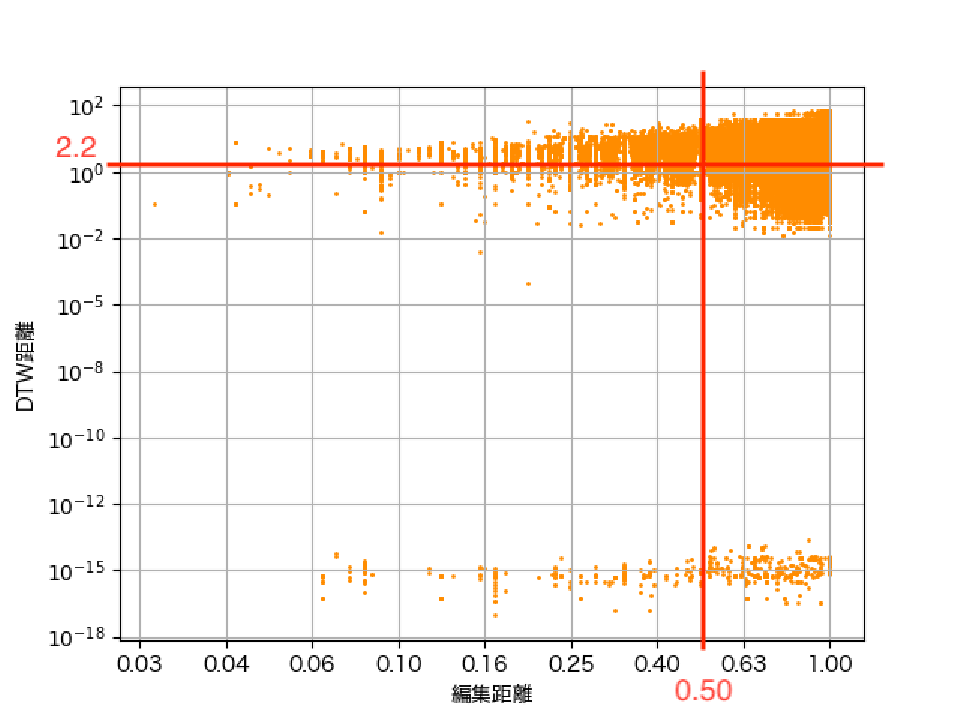
\includegraphics[width=1.0\linewidth]{Okamoto_fig/out-all-nolimit.pdf}
	\caption{DTW距離と編集距離の関係性を示した散布図}
	\label{fig:out-nolimit}
\end{figure}
%------------------------

%-------------------------
\begin{figure*}[t]
    \begin{tabular}{cc}
  \begin{minipage}[t]{0.45\linewidth}
    \centering
	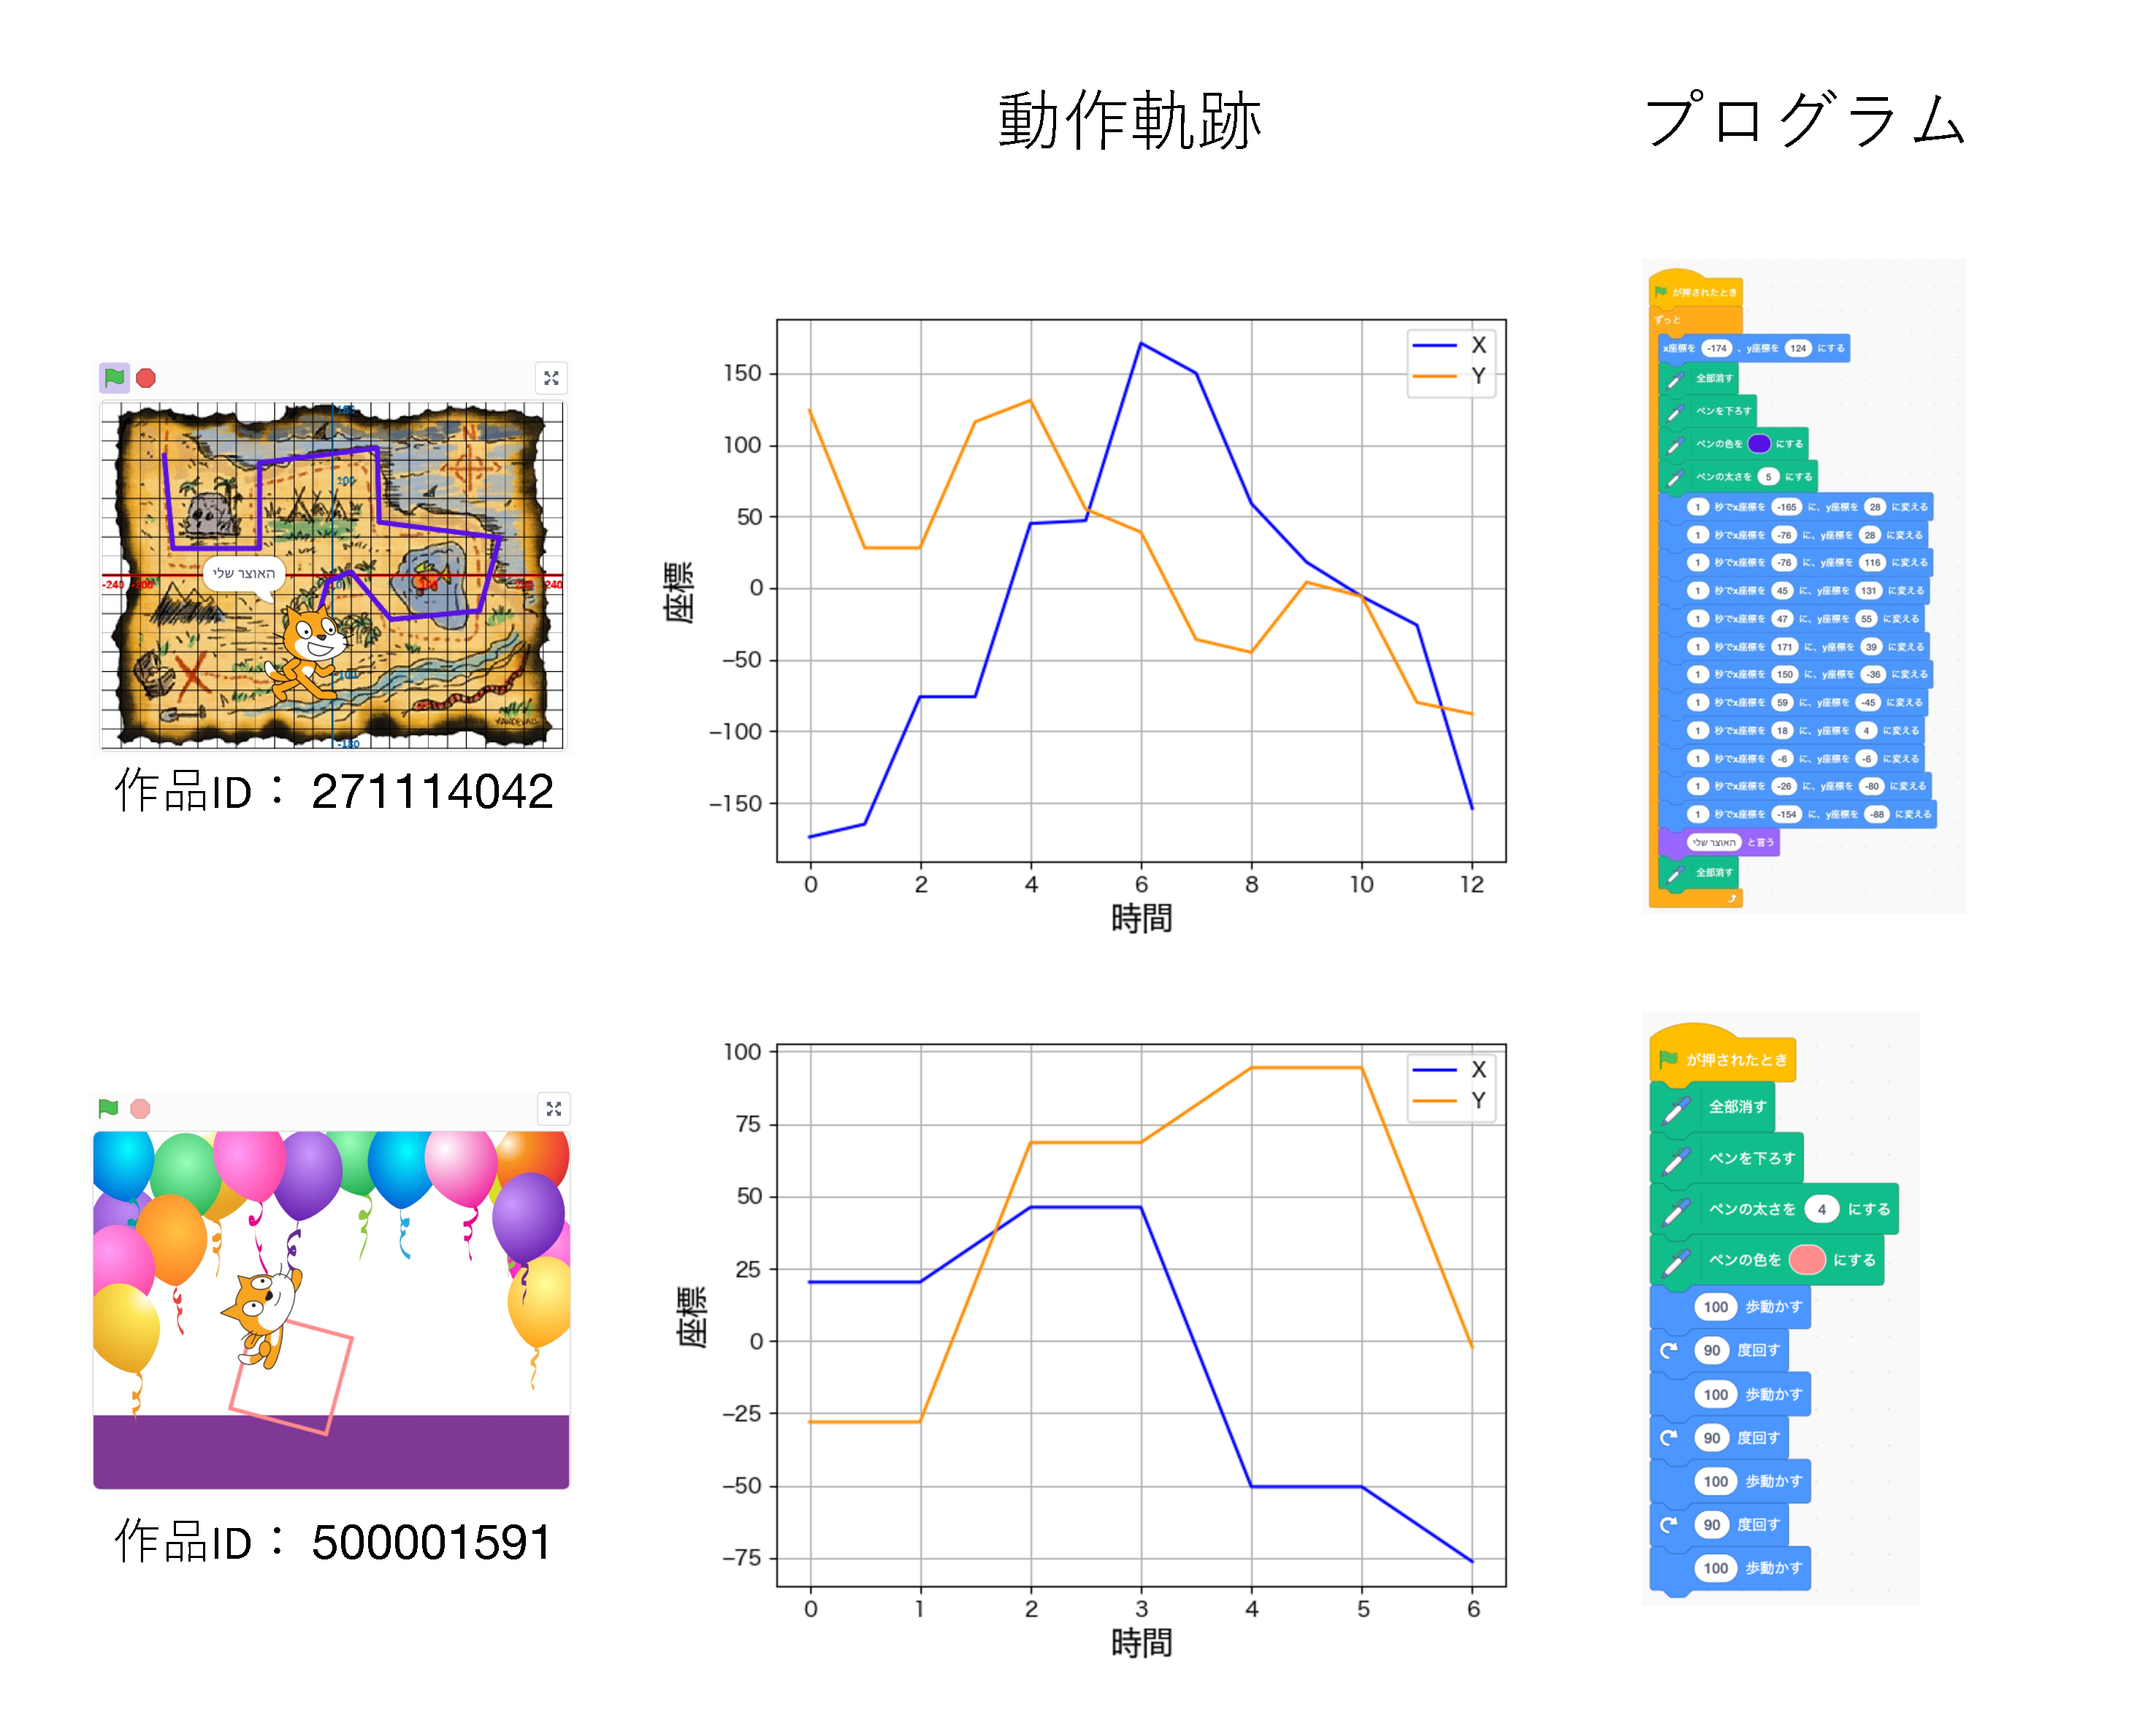
\includegraphics[keepaspectratio, scale=0.14]{Okamoto_fig/quadrant-1.pdf}
    \caption{第1象限に含まれる作品対の事例}
    \label{fig:distance-boxplot1}
  \end{minipage}
  \begin{minipage}[t]{0.45\linewidth}
    \centering
	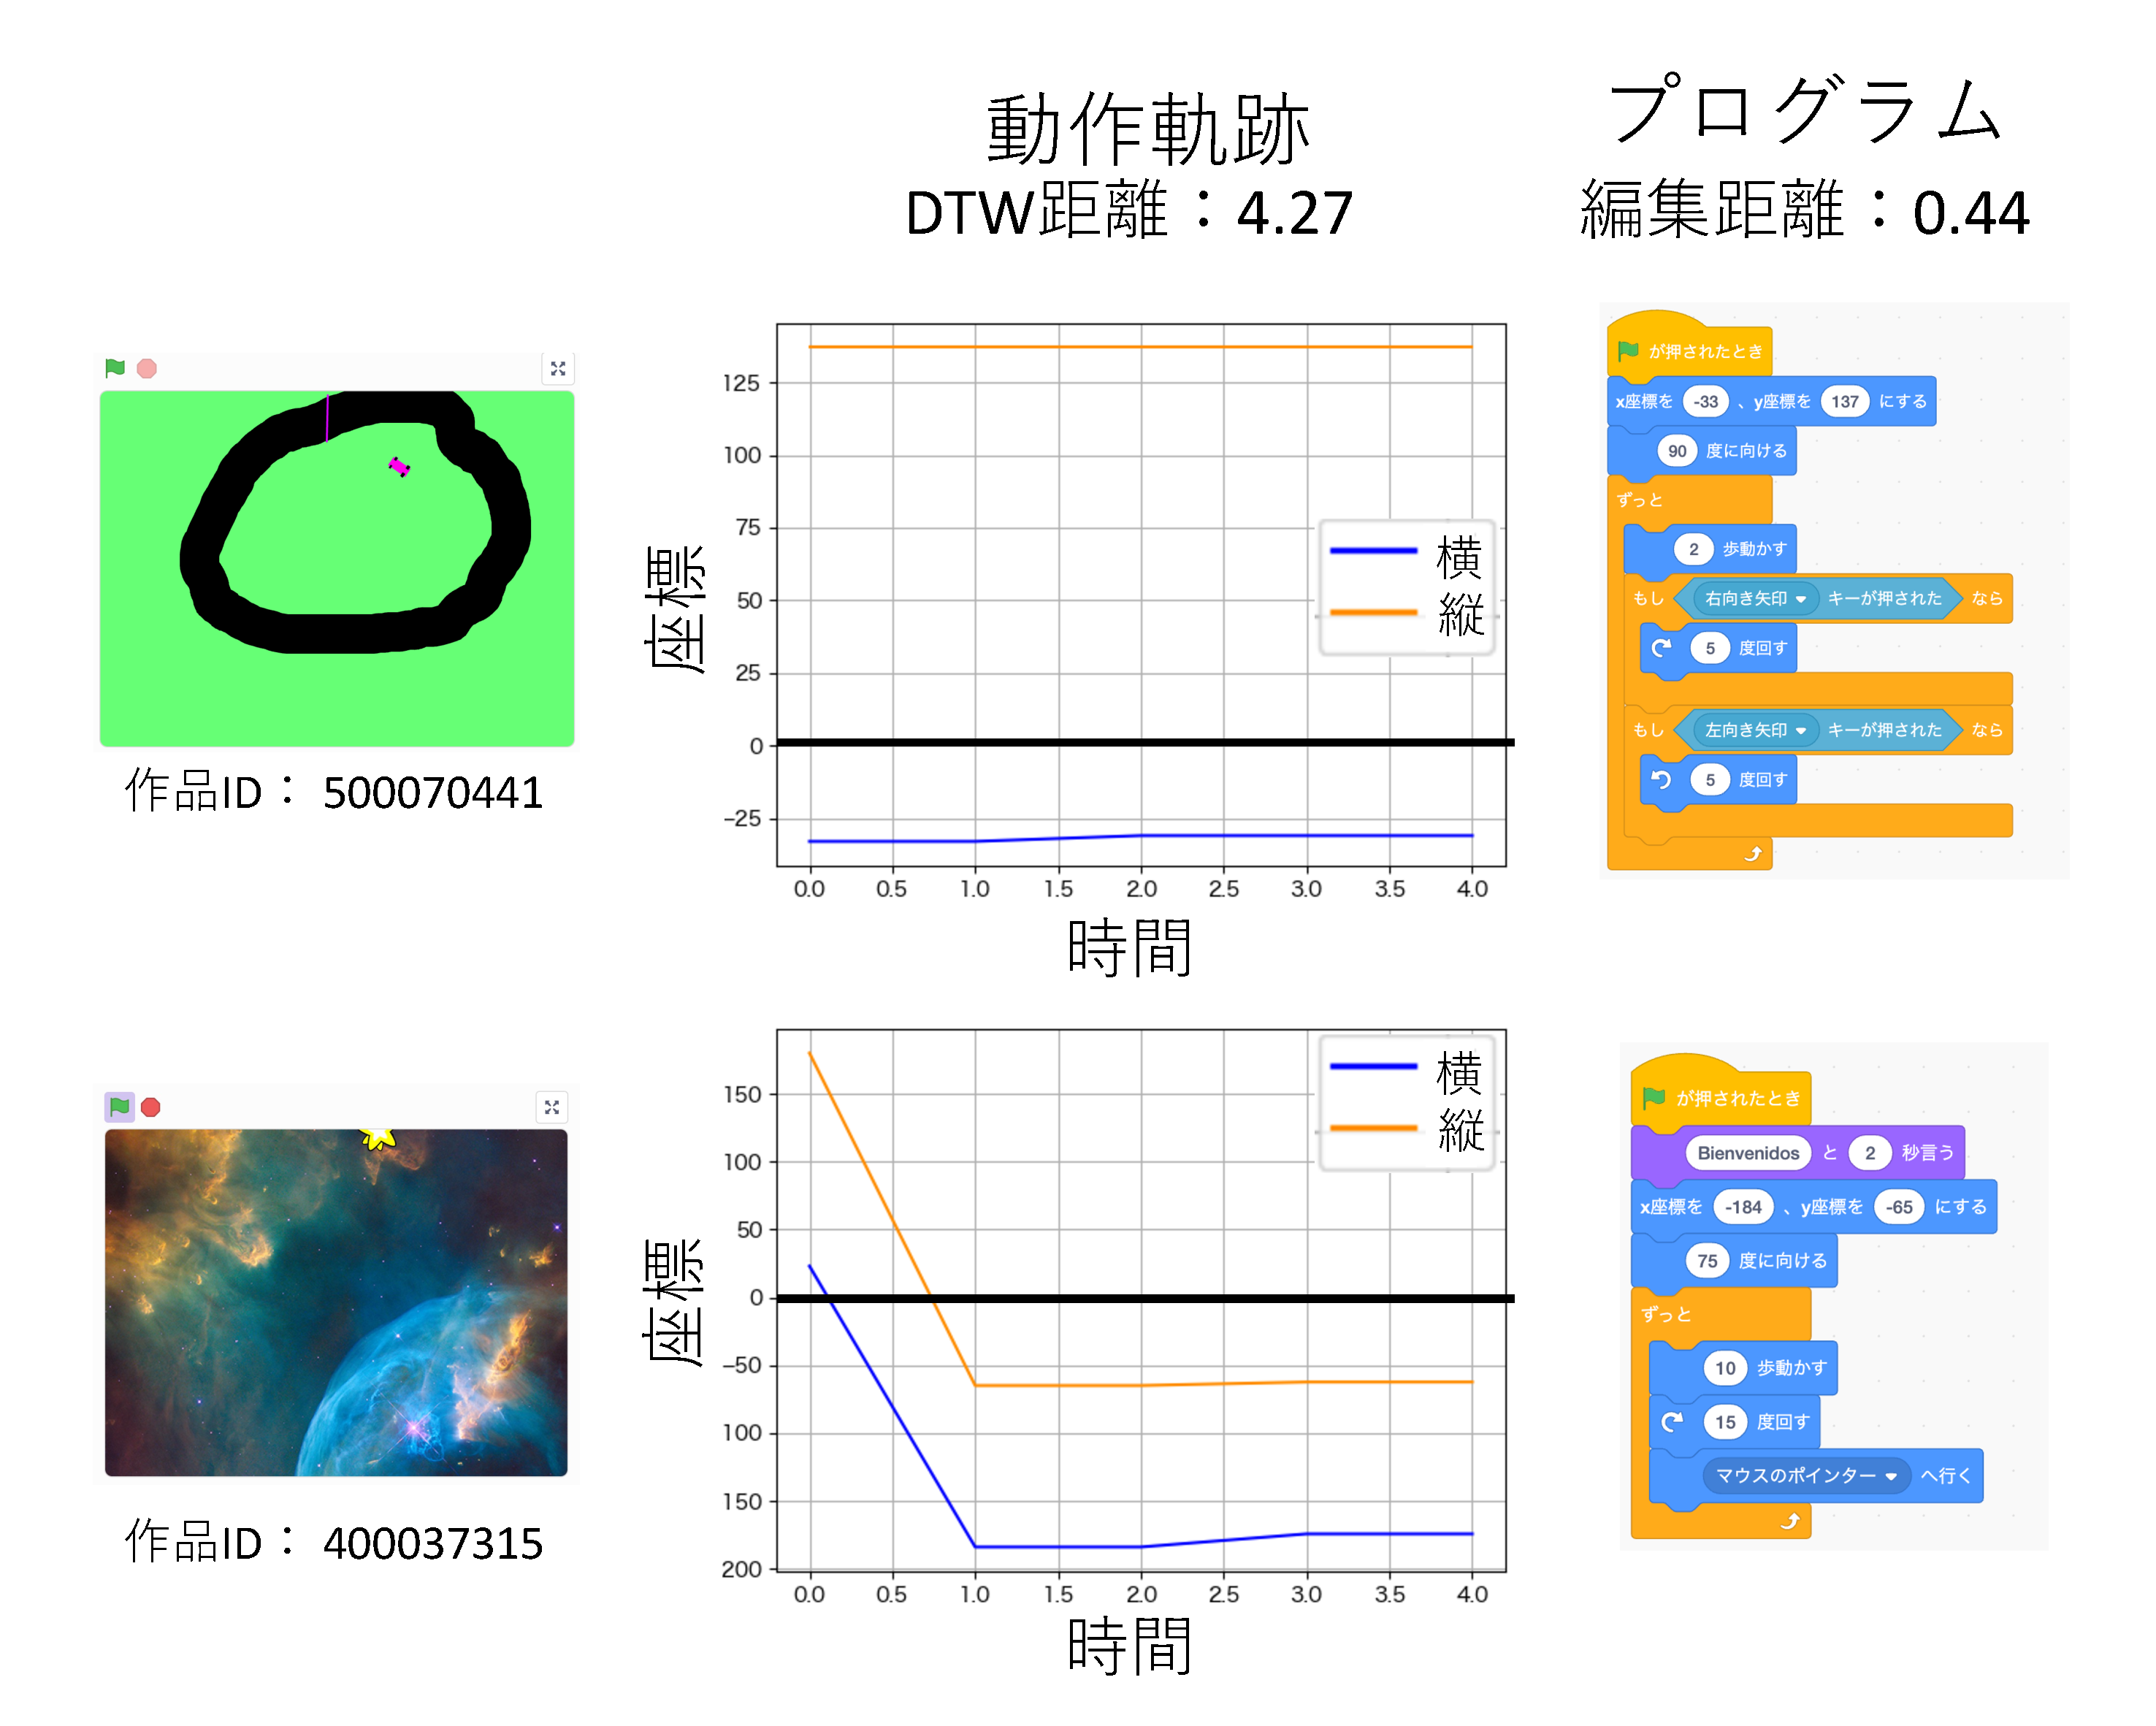
\includegraphics[keepaspectratio, scale=0.14]{Okamoto_fig/quadrant-2.pdf}
	\caption{第2象限に含まれる作品対の事例}
	\label{fig:distance-boxplot2}
  \end{minipage}
    \end{tabular}

    \begin{tabular}{cc}

  \begin{minipage}[b]{0.45\linewidth}
    \centering
	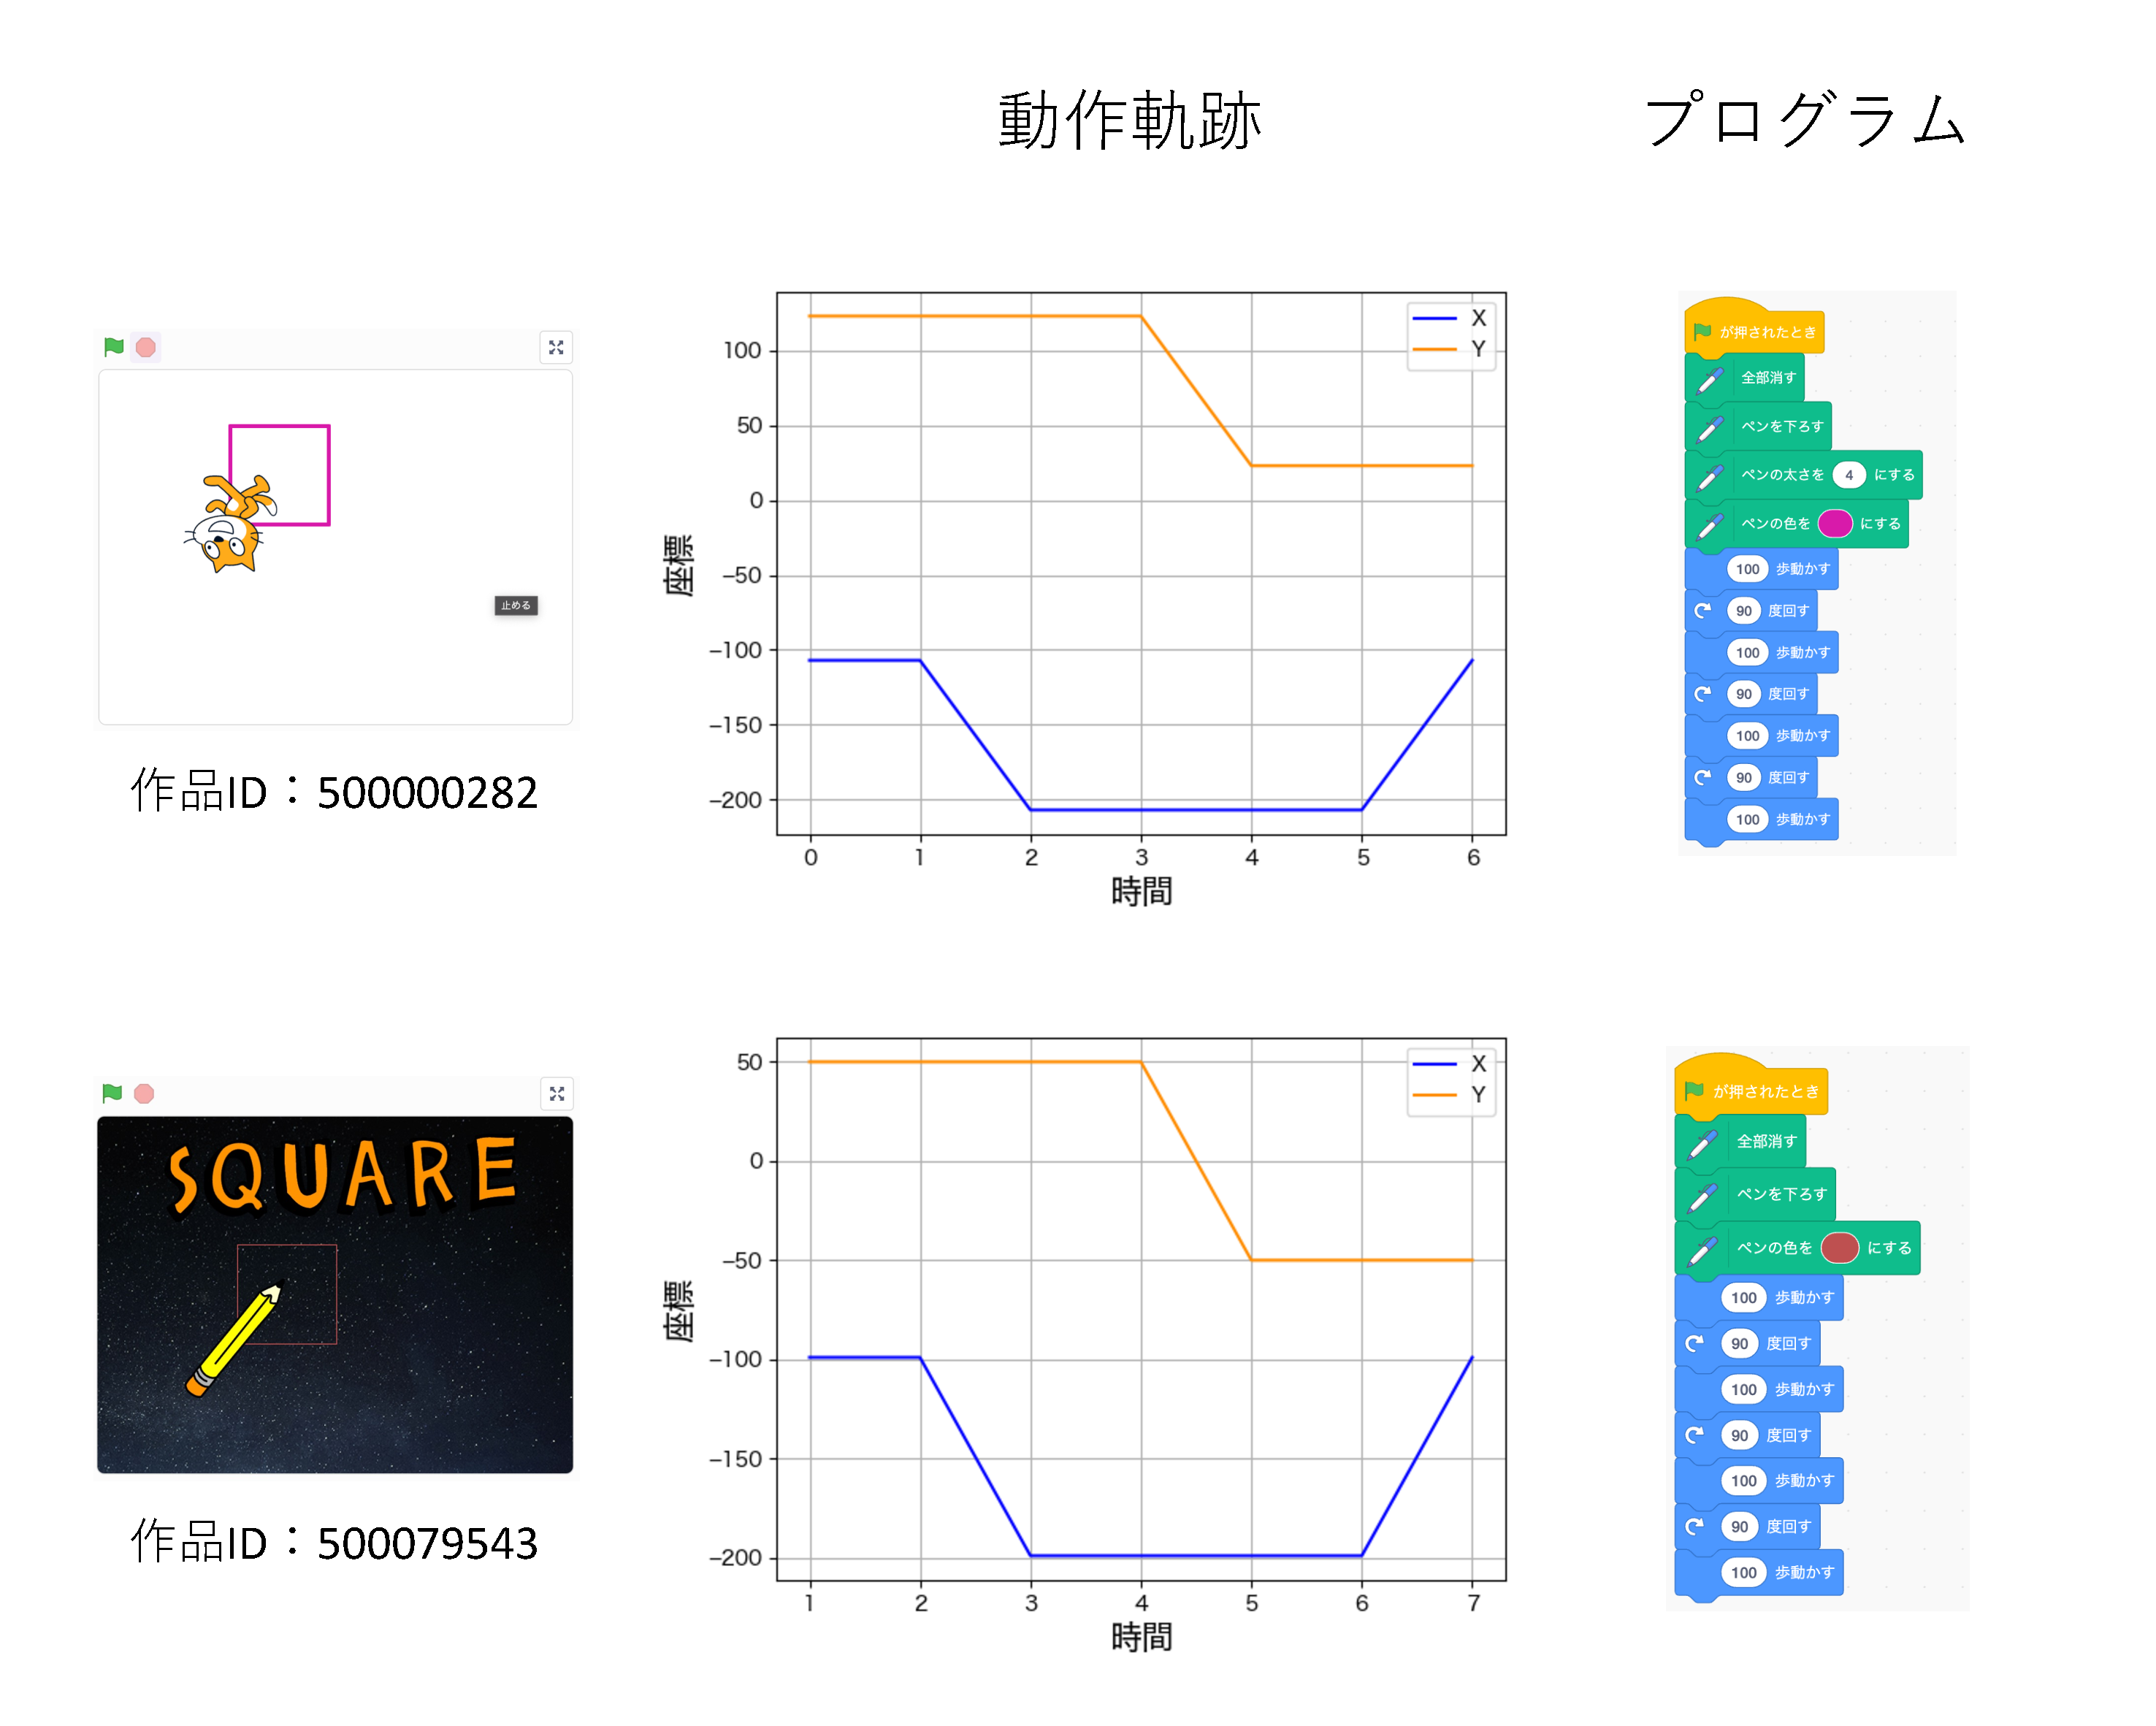
\includegraphics[keepaspectratio, scale=0.14]{Okamoto_fig/quadrant-3.pdf}
	\caption{第3象限に含まれる作品対の事例}
	\label{fig:distance-boxplot3}
  \end{minipage}
  \begin{minipage}[b]{0.45\linewidth}
    \centering
	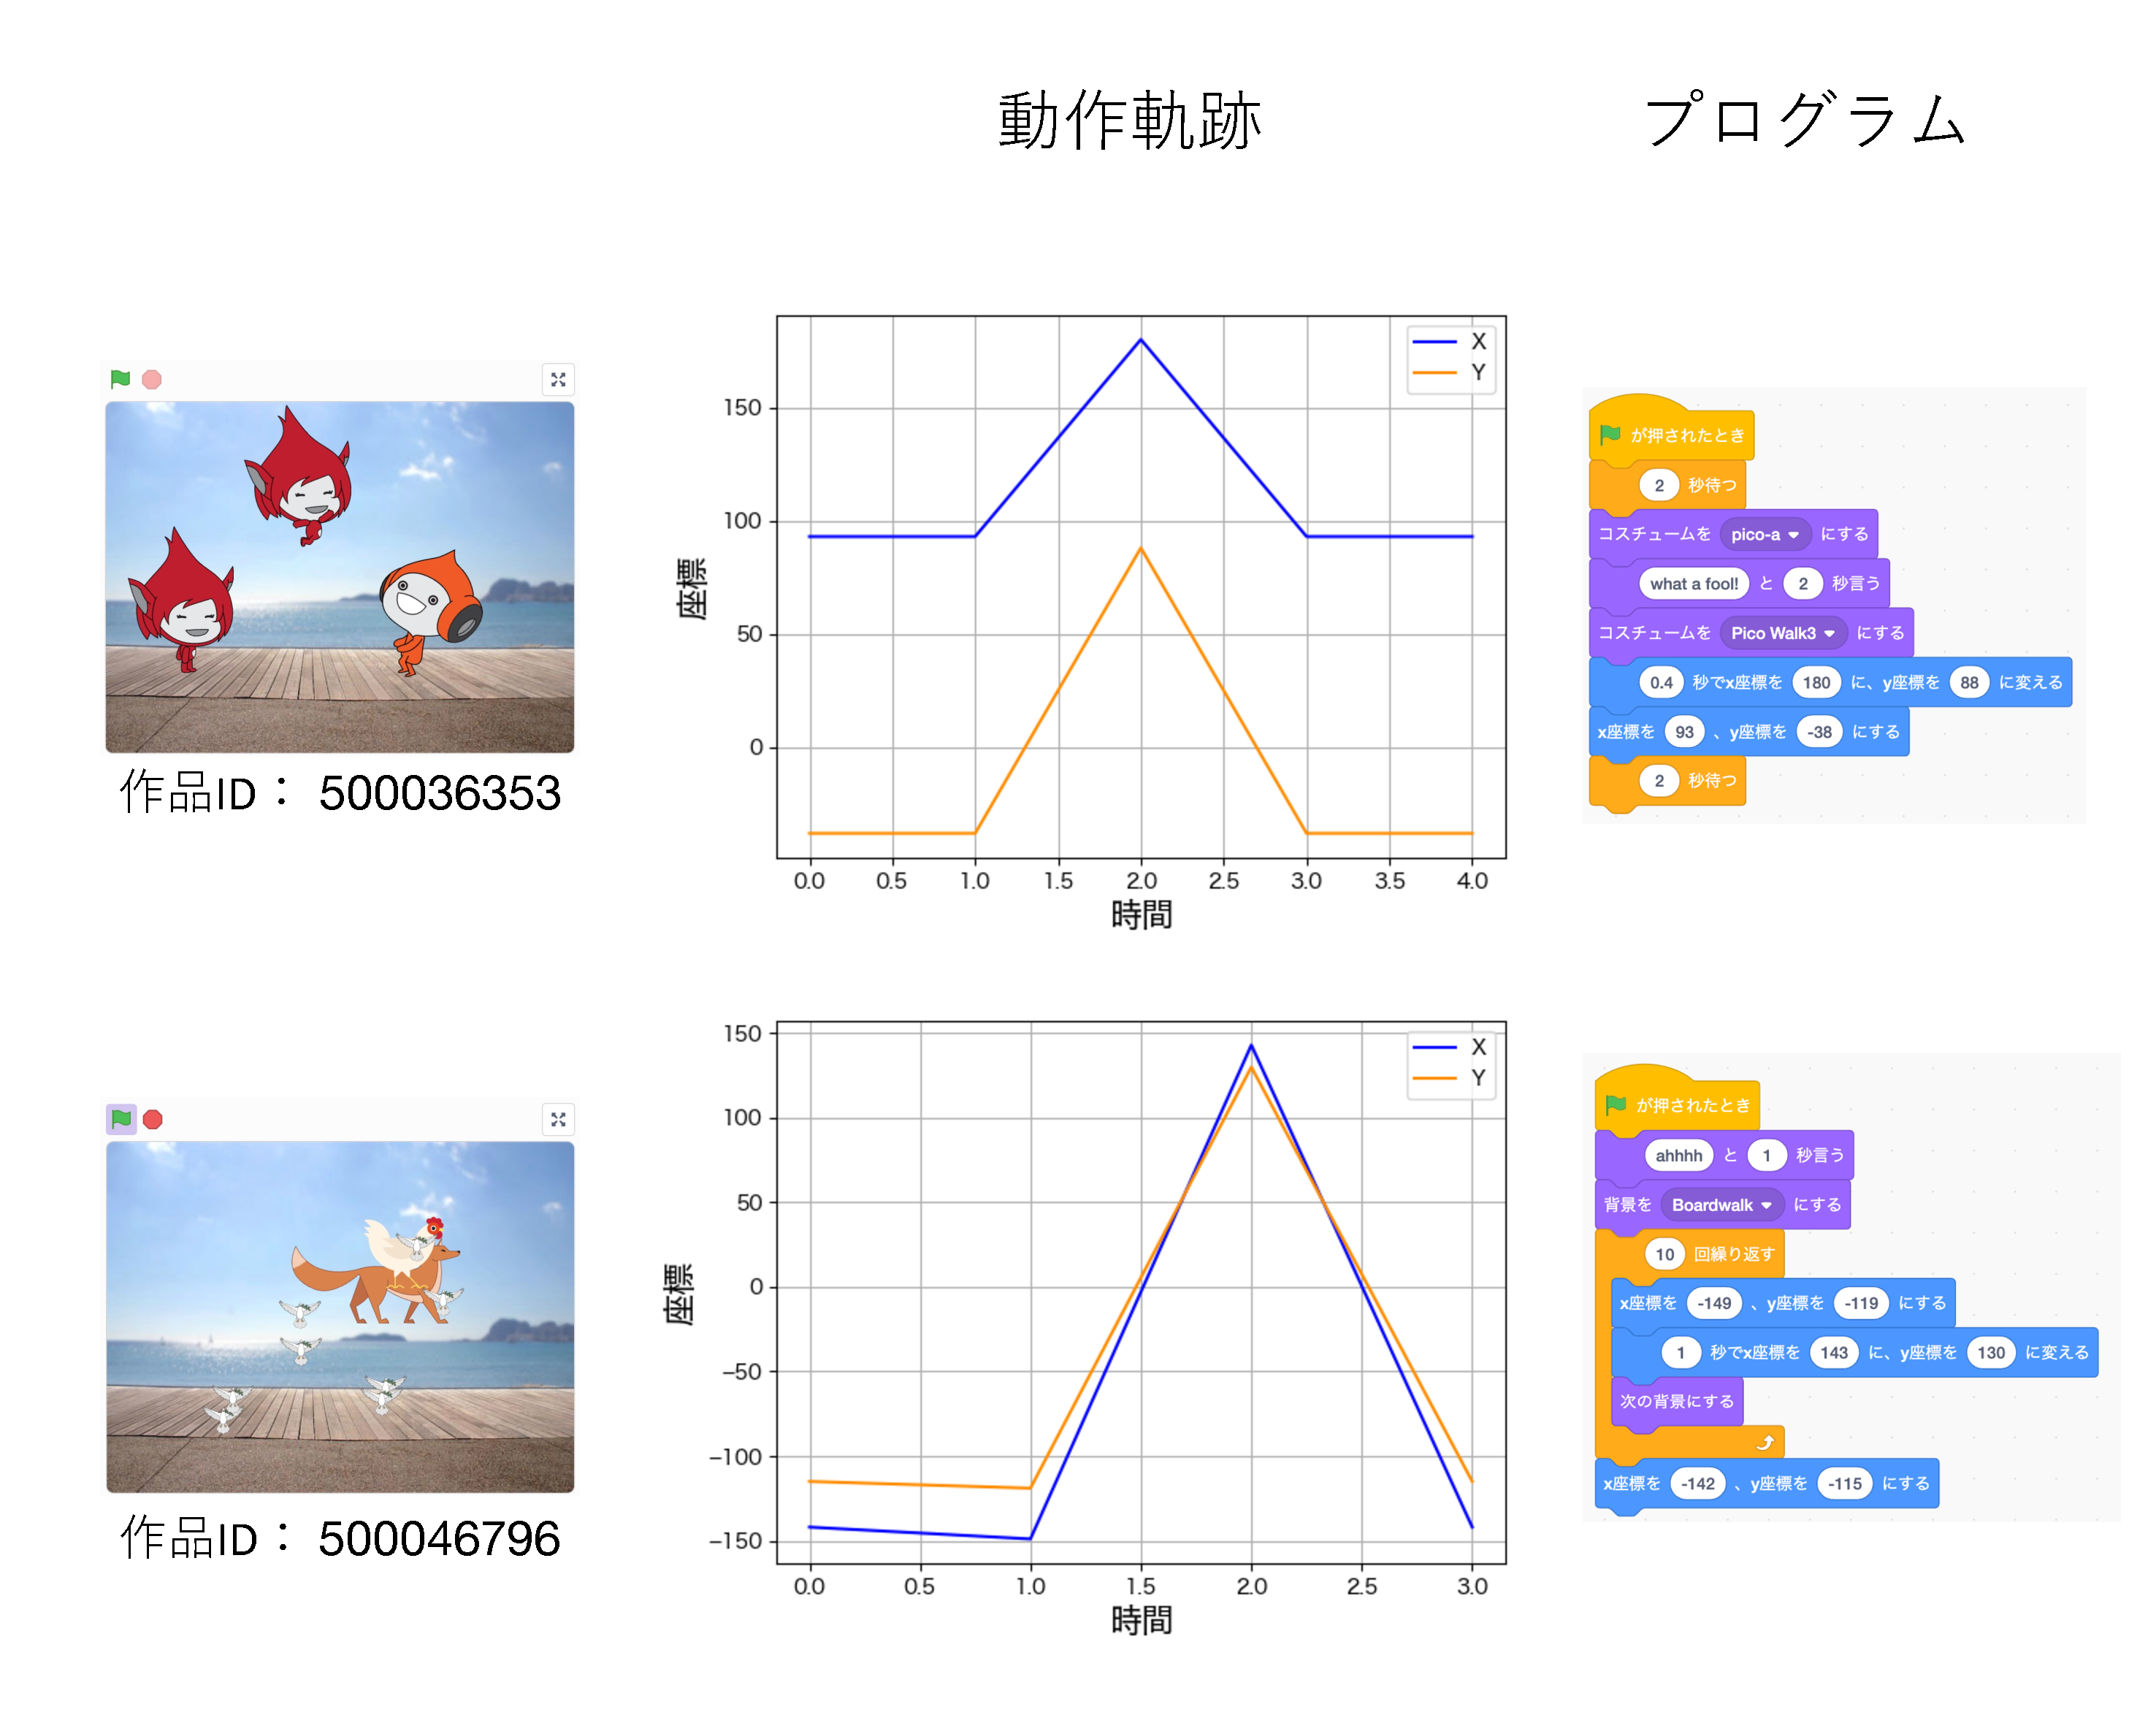
\includegraphics[keepaspectratio, scale=0.14]{Okamoto_fig/quadrant-4.pdf}
	\caption{第4象限に含まれる作品対の事例}
	\label{fig:distance-boxplot4}
  \end{minipage}
    \end{tabular}
\end{figure*}
%-------------------------

図\ref{fig:out-nolimit}は,分析対象とする4,000作品を総当たりに編集距離とDTW距離を計測した結果を散布図で示す.横軸は編集距離、縦軸はDTW距離を示す.それぞれの軸は対数表記している.散布図の1点は,2つの作品間の類似度を計測した作品対の結果を表す.また,編集距離とDTW距離の境界値を赤線で示す.この境界線に基づき,4000作品の中から類似度を算出できた7,595,815作品対を4つに分類する.
%散布図中の第2象限は動作軌跡もプログラムも類似しない,第2象限は動作軌跡は類似しないが,プログラムは類似する,第3象限は動作軌跡もプログラムも類似する,第4象限は動作軌跡は類似するが,プログラムが類似しないことをそれぞれ意味する.
図\ref{fig:distance-boxplot1},図\ref{fig:distance-boxplot2},図\ref{fig:distance-boxplot3},図\ref{fig:distance-boxplot4}は第1象限〜第4象限までに分類されたそれぞれの作品事例の動作軌跡(折れ線グラフ)とプログラムを示す.折れ線グラフは青線が横方向の移動,黄線が縦方向の移動で示し,中央の太線以上の値は,横軸に右方向,縦軸に上方向の移動を示す.続いて,図\ref{fig:out-nolimit}の散布図を象限別の知見を事例と併せて述べる.

\noindent\textbf{第1象限:}図\ref{fig:distance-boxplot1}は動作軌跡とプログラムが乖離する第1象限の作品対の事例を示す.動作軌跡はそれぞれ横方向と縦方向の移動は類似していない.また,プログラムからも青色の座標移動ブロックや,緑色のペンブロックを利用しているため同じ役割を持つブロックを多く利用しているが,上の作品(ID: 271114042)ではループを使用し,下の作品(ID: 500001591)では座標移動ブロックの中で2種のブロックを使い分けているためプログラム構造は類似していない.

\noindent\textbf{第2象限:}図\ref{fig:distance-boxplot2}は動作軌跡は類似しないが,プログラムが類似する第2象限の作品対の事例を示す.動作軌跡はそれぞれ横方向も縦方向も動作が異なるが,プログラムはいずれもループを使用し,その他も同じ種類のブロックを使用しているため類似している.このようにプログラムは類似するが,DTW距離が異なるのは図\ref{fig:pattern1}の事例にも示したように,ブロックの引数,演算子が異なることが多い.

\noindent\textbf{第3象限:}図\ref{fig:distance-boxplot3}は動作軌跡とプログラムがそれぞれ類似している第3象限の作品対の事例を示す.動作軌跡は横方向も縦方向も動作が極めて類似し,プログラムに使用するブロックの種類や数も極めて一致している.散布図の下部に集中して一部の作品対が集中しているように見えるが,対数表記していることが影響している.ただし,作品が直線移動のような単調な動作軌跡であれば,DTW距離が小さくなる.

\noindent\textbf{第4象限:}図\ref{fig:distance-boxplot4}は動作軌跡は類似するが,プログラムが類似しない第4象限の作品対の事例を示す.動作軌跡は,座標のずれはあるが動作は類似している.また,プログラムからは,下の作品(ID: 500046796)ではループしているのに対し,上の作品(ID: 500046796)では用いていない点から類似していないことがわかる.このようにDTW距離は小さく,編集距離が大きい第4象限の作品対は,多様な実装方法を収集するために有効であると示唆される.

%図中の1点は1つの作品対であることを表す.また,\ref{subsec:approach}で示した境界値を図中の線で示しており,この境界線に基づいて作品を4種類に分類した.






\subsubsection{分析1:分類別の統計量}

表\ref{table:programs-classification}は4つの各象限に分類された作品対の数を示す.本ケーススタディで取得した作品対の合計数は7,595,815件であり,移動軌跡,プログラムともに類似する作品は約1\%,移動軌跡もプログラムも類似しない作品は約70\%であった.特に動作軌跡は類似するがプログラムが類似しない作品が約28\%も存在し,Scratchでは類似作品が多様な実装方法で作成されている.

% \todo{いらない気がする}表\ref{table:program-classification}は4つに分類された作品対のうち,それぞれの分類に含まれる作品の数を示している.本ケーススタディで分類した作品数は4000であるため,表\ref{table:programs-classification}より,分類された作品の数に大きな違いはないことがわかる.

% 表\ref{table:program-length}は4つに分類された作品のプログラムに含まれるブロック数(ブロック長)の平均値を示している.この結果より,4つに分類された作品群の間で,ブロック長には大きな違いがないことがわかる.

%-------------------
\begin{table}[t]
    \centering
    \caption{分類別作品対の数の比較}
    \begin{tabular}{c|l|r|r}
        \hline
        \multicolumn{2}{c|}{}& \multicolumn{2}{c}{プログラム} \\ \cline{3-4}
        \multicolumn{2}{c|}{}& \multicolumn{1}{c|}{類似する} & \multicolumn{1}{c}{類似しない} \\
        \hline
        動作&類似しない & 41,877 & 5,293,007 \\
        軌跡&類似する & 98,408 & 2,162,523 \\ \cline{2-4}
        \hline
    \end{tabular}
%    \captionsetup{skip=5pt}
    \label{table:programs-classification}

% \vspace{2mm}

%     \centering
%     \caption{分類別作品数の比較}
%     \begin{tabular}{c|l|r|r}
%         \hline
%         \multicolumn{2}{c|}{}& \multicolumn{2}{c}{プログラム} \\ \cline{3-4}
%         \multicolumn{2}{c|}{}& \multicolumn{1}{c|}{類似する} & \multicolumn{1}{c}{類似しない} \\
%         \hline
%         動作&類似しない & 3,017 & 3,889 \\
%         軌跡&類似する & 2,842 & 3,603 \\
%         \hline
%     \end{tabular}
%     \captionsetup{skip=5pt}
%     \label{table:program-classification}

% \vspace{2mm}

%     \centering
%     \caption{分類別ブロック長平均値の比較}
%     \begin{tabular}{c|l|r|r}
%         \hline
%         \multicolumn{2}{c|}{}& \multicolumn{2}{c}{プログラム} \\ \cline{3-4}
%         \multicolumn{2}{c|}{}& \multicolumn{1}{c|}{類似する} & \multicolumn{1}{c}{類似しない} \\
%         \hline
%         動作&類似しない & 15.4 & 18.0 \\
%         軌跡&類似する & 15.5 & 16.7 \\
%         \hline
%     \end{tabular}
%     \captionsetup{skip=5pt}
%     \label{table:program-length}
\end{table}
%-------------------

\subsubsection{分析2:分類別のDTW距離の分布}

図\ref{fig:dtw-boxplot}は,4つの各象限に分類された作品対のDTW距離の分布を示した箱ひげ図を示す.
%外れ値は描画していない.
第1象限と第2象限はDTW距離の中央値はそれぞれ6.43と5.41であり,第3象限と第4象限はDTW距離の中央値はそれぞれ1.41と2.00である.第1象限と第2象限,および第3象限と第4象限のDTW距離の分布には,統計的有意差があることを確認した(マンホイットニーのU検定,p値$<$0.05).また,Cohen's d\cite{cohen2013statistical}の効果量を測定した結果,それぞれ0.22と0.49を得られ,分布間の効果量は小程度であった.第3象限と第4象限の作品対はプログラムの類似度は極めて異なるが,それが移動軌跡に与える影響は少ないことが示唆される.


% 第3象限と第4象限の作品対は共にDTW距離が小さいが,編集距離が大きい第4象限に比べて,第3象限の方がDTW距離が小さいため,作品として類似している.\todo{効果量次第?効果量が小さい場合は,DTWが小さくてもプログラムが違うので多様性のある実装が多い,みたいなことを言う.}

\subsubsection{分析3:分類別の編集距離の分布}
図\ref{fig:distance-boxplot}は,4つの各象限に分類された作品対の編集距離の分布を示した箱ひげ図を示す.
%外れ値は描画していない.
第1象限と第4象限は編集距離の中央値はどちらも0.91であり,第2象限と第3象限はDTW距離の中央値はそれぞれ0.46と0.44である.第1象限と第4象限,および第2象限と第3象限の編集距離の分布には,統計的有意差があることを確認した(マンホイットニーのU検定,p値$<$0.05).また,Cohen's d\cite{cohen2013statistical}の効果量を測定した結果,それぞれ0.024と0.18を得られ,分布間の効果量は小程度であった.第2象限と第3象限の移動軌跡の類似度は極めて異なるが,プログラムは類似してしまうため作品検索においてノイズとなり得るが,第2象限の作品対は全体の作品対の約1\%であるため大きな課題ではない.

% 編集距離の分布には確実な差異が存在することが示されたが,その差異は実質的には小さいことが示唆される.

% 第象限と第3象限の作品対は共に編集距離が小さいが,DTW距離が大きい第2象限に比べて,第3象限の方が編集距離が小さいため,作品として類似している.

% \todo{効果量次第?効果量が小さい場合は,プログラムが似通っていてもDTWは違うので,検索が難しい,みたいなことを言う?}

%-------------------------
\begin{figure}[t]
	\centering
	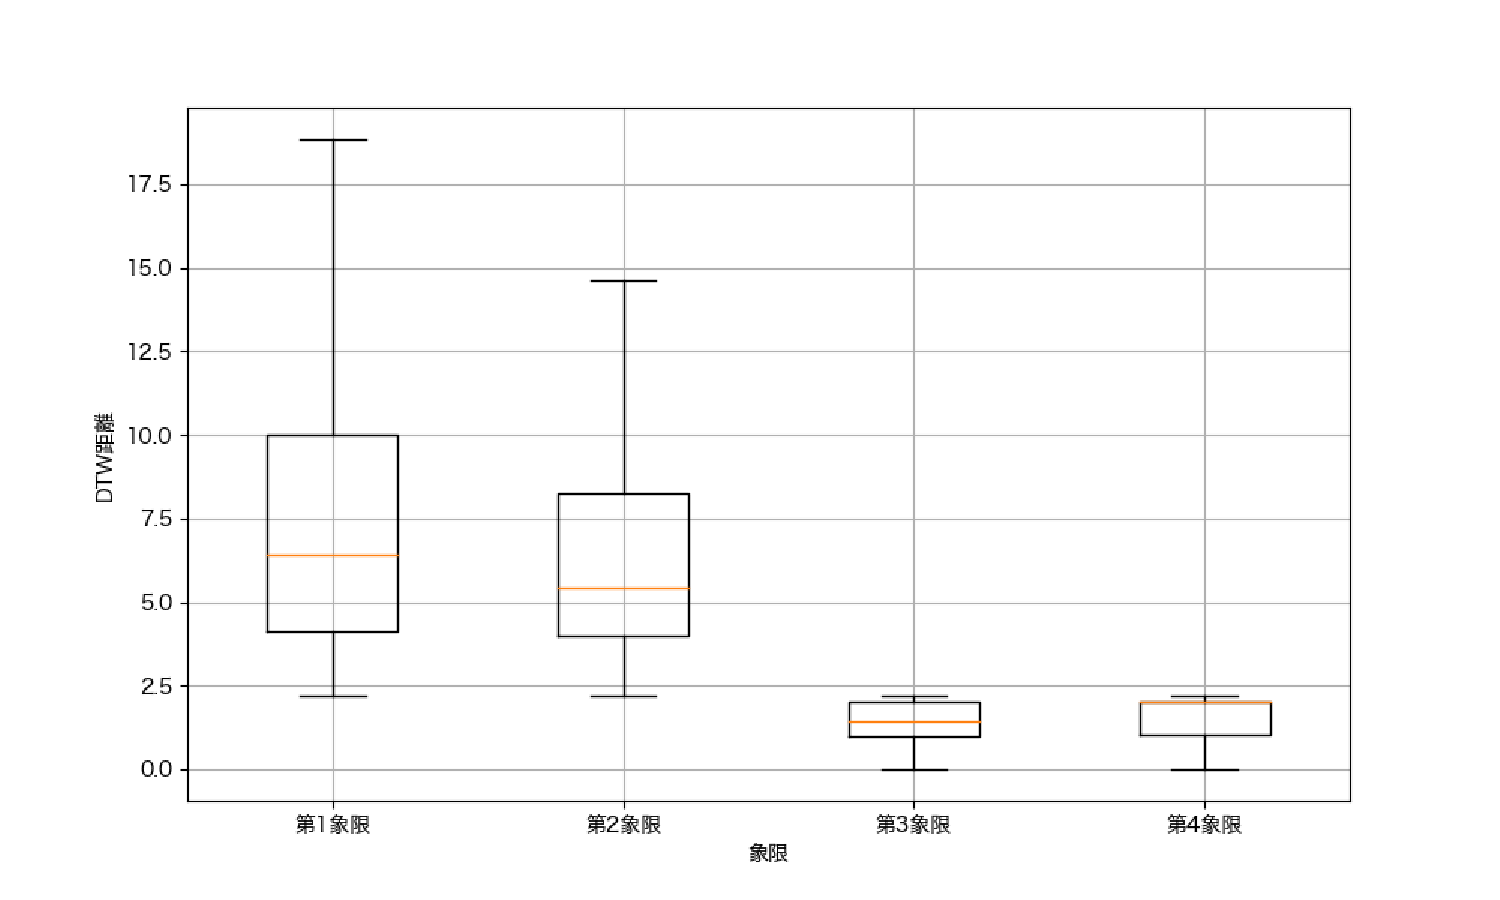
\includegraphics[width=1.0\linewidth]{Okamoto_fig/DTW-out.pdf}
	\caption{分類別にDTW距離の分布を示した箱ひげ図}
	\label{fig:dtw-boxplot}

	\centering
	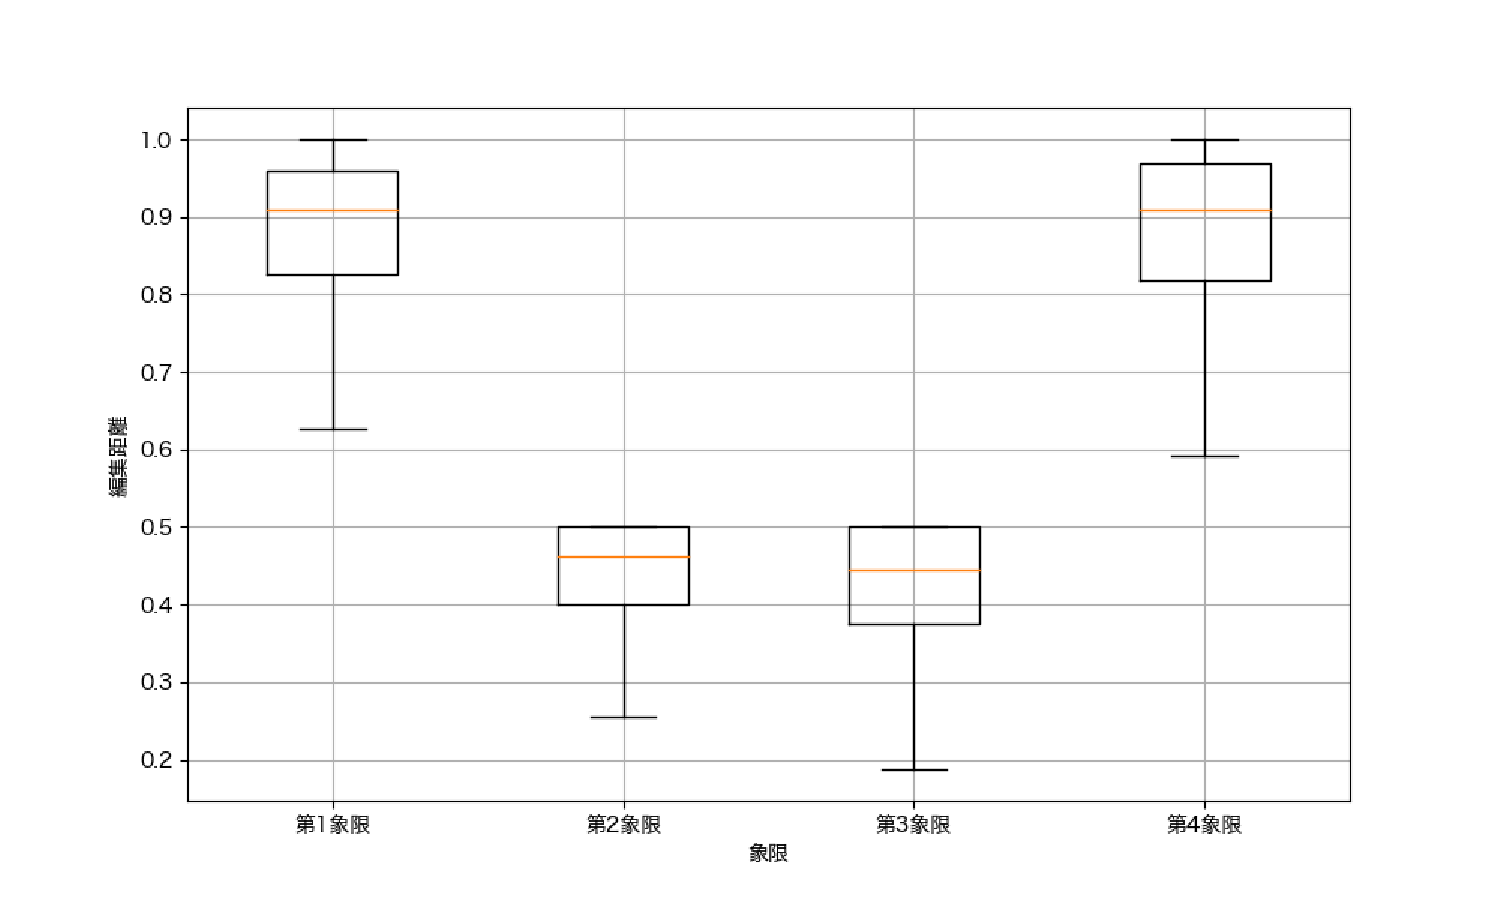
\includegraphics[width=1.0\linewidth]{Okamoto_fig/distance-out.pdf}
	\caption{分類別に編集距離の分布を示した箱ひげ図}
	\label{fig:distance-boxplot}
\end{figure}
%-------------------------

% % プログラムも動作軌跡も類似しない作品対
% \begin{figure}[t]
% 	\centering
% 	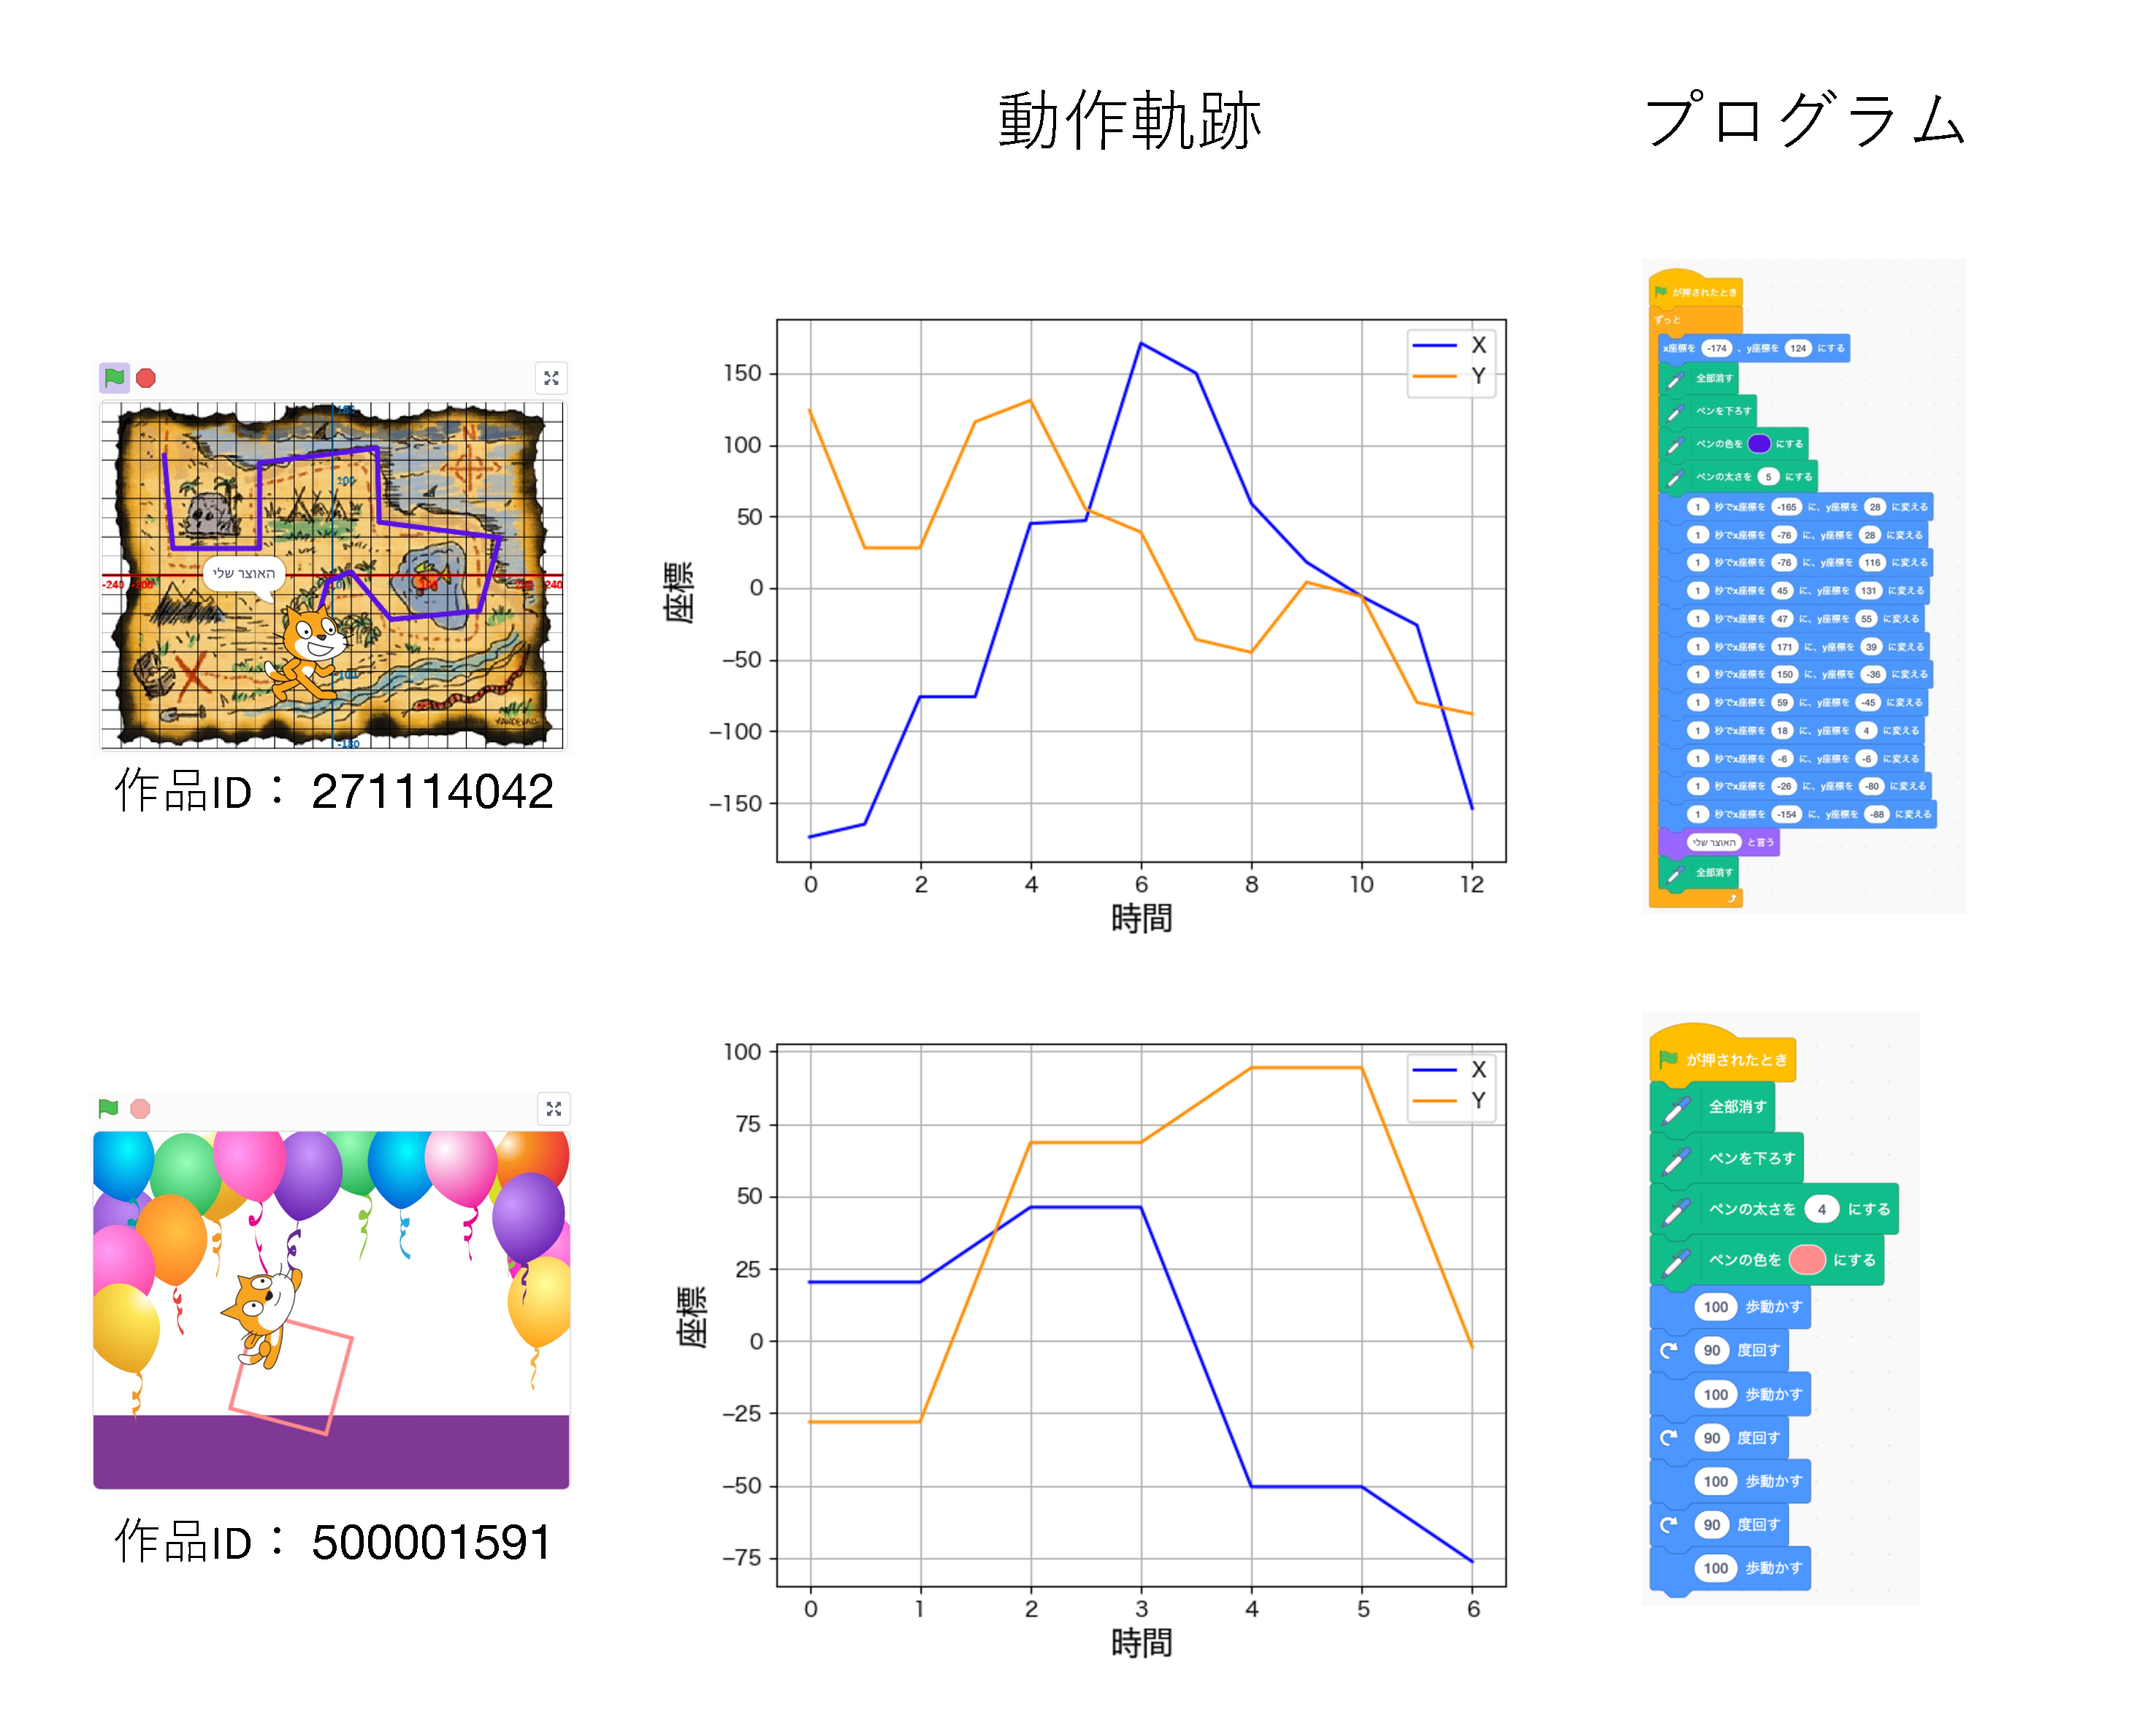
\includegraphics[width=1.0\linewidth]{Okamoto_fig/quadrant-1.pdf}
% 	\caption{DTW距離が7.92,編集距離が0.81の作品対}
% 	\label{fig:distance-boxplot}
% \end{figure}

% % プログラムは類似するが,動作軌跡は類似しない作品対
% \begin{figure}[t]
% 	\centering
% 	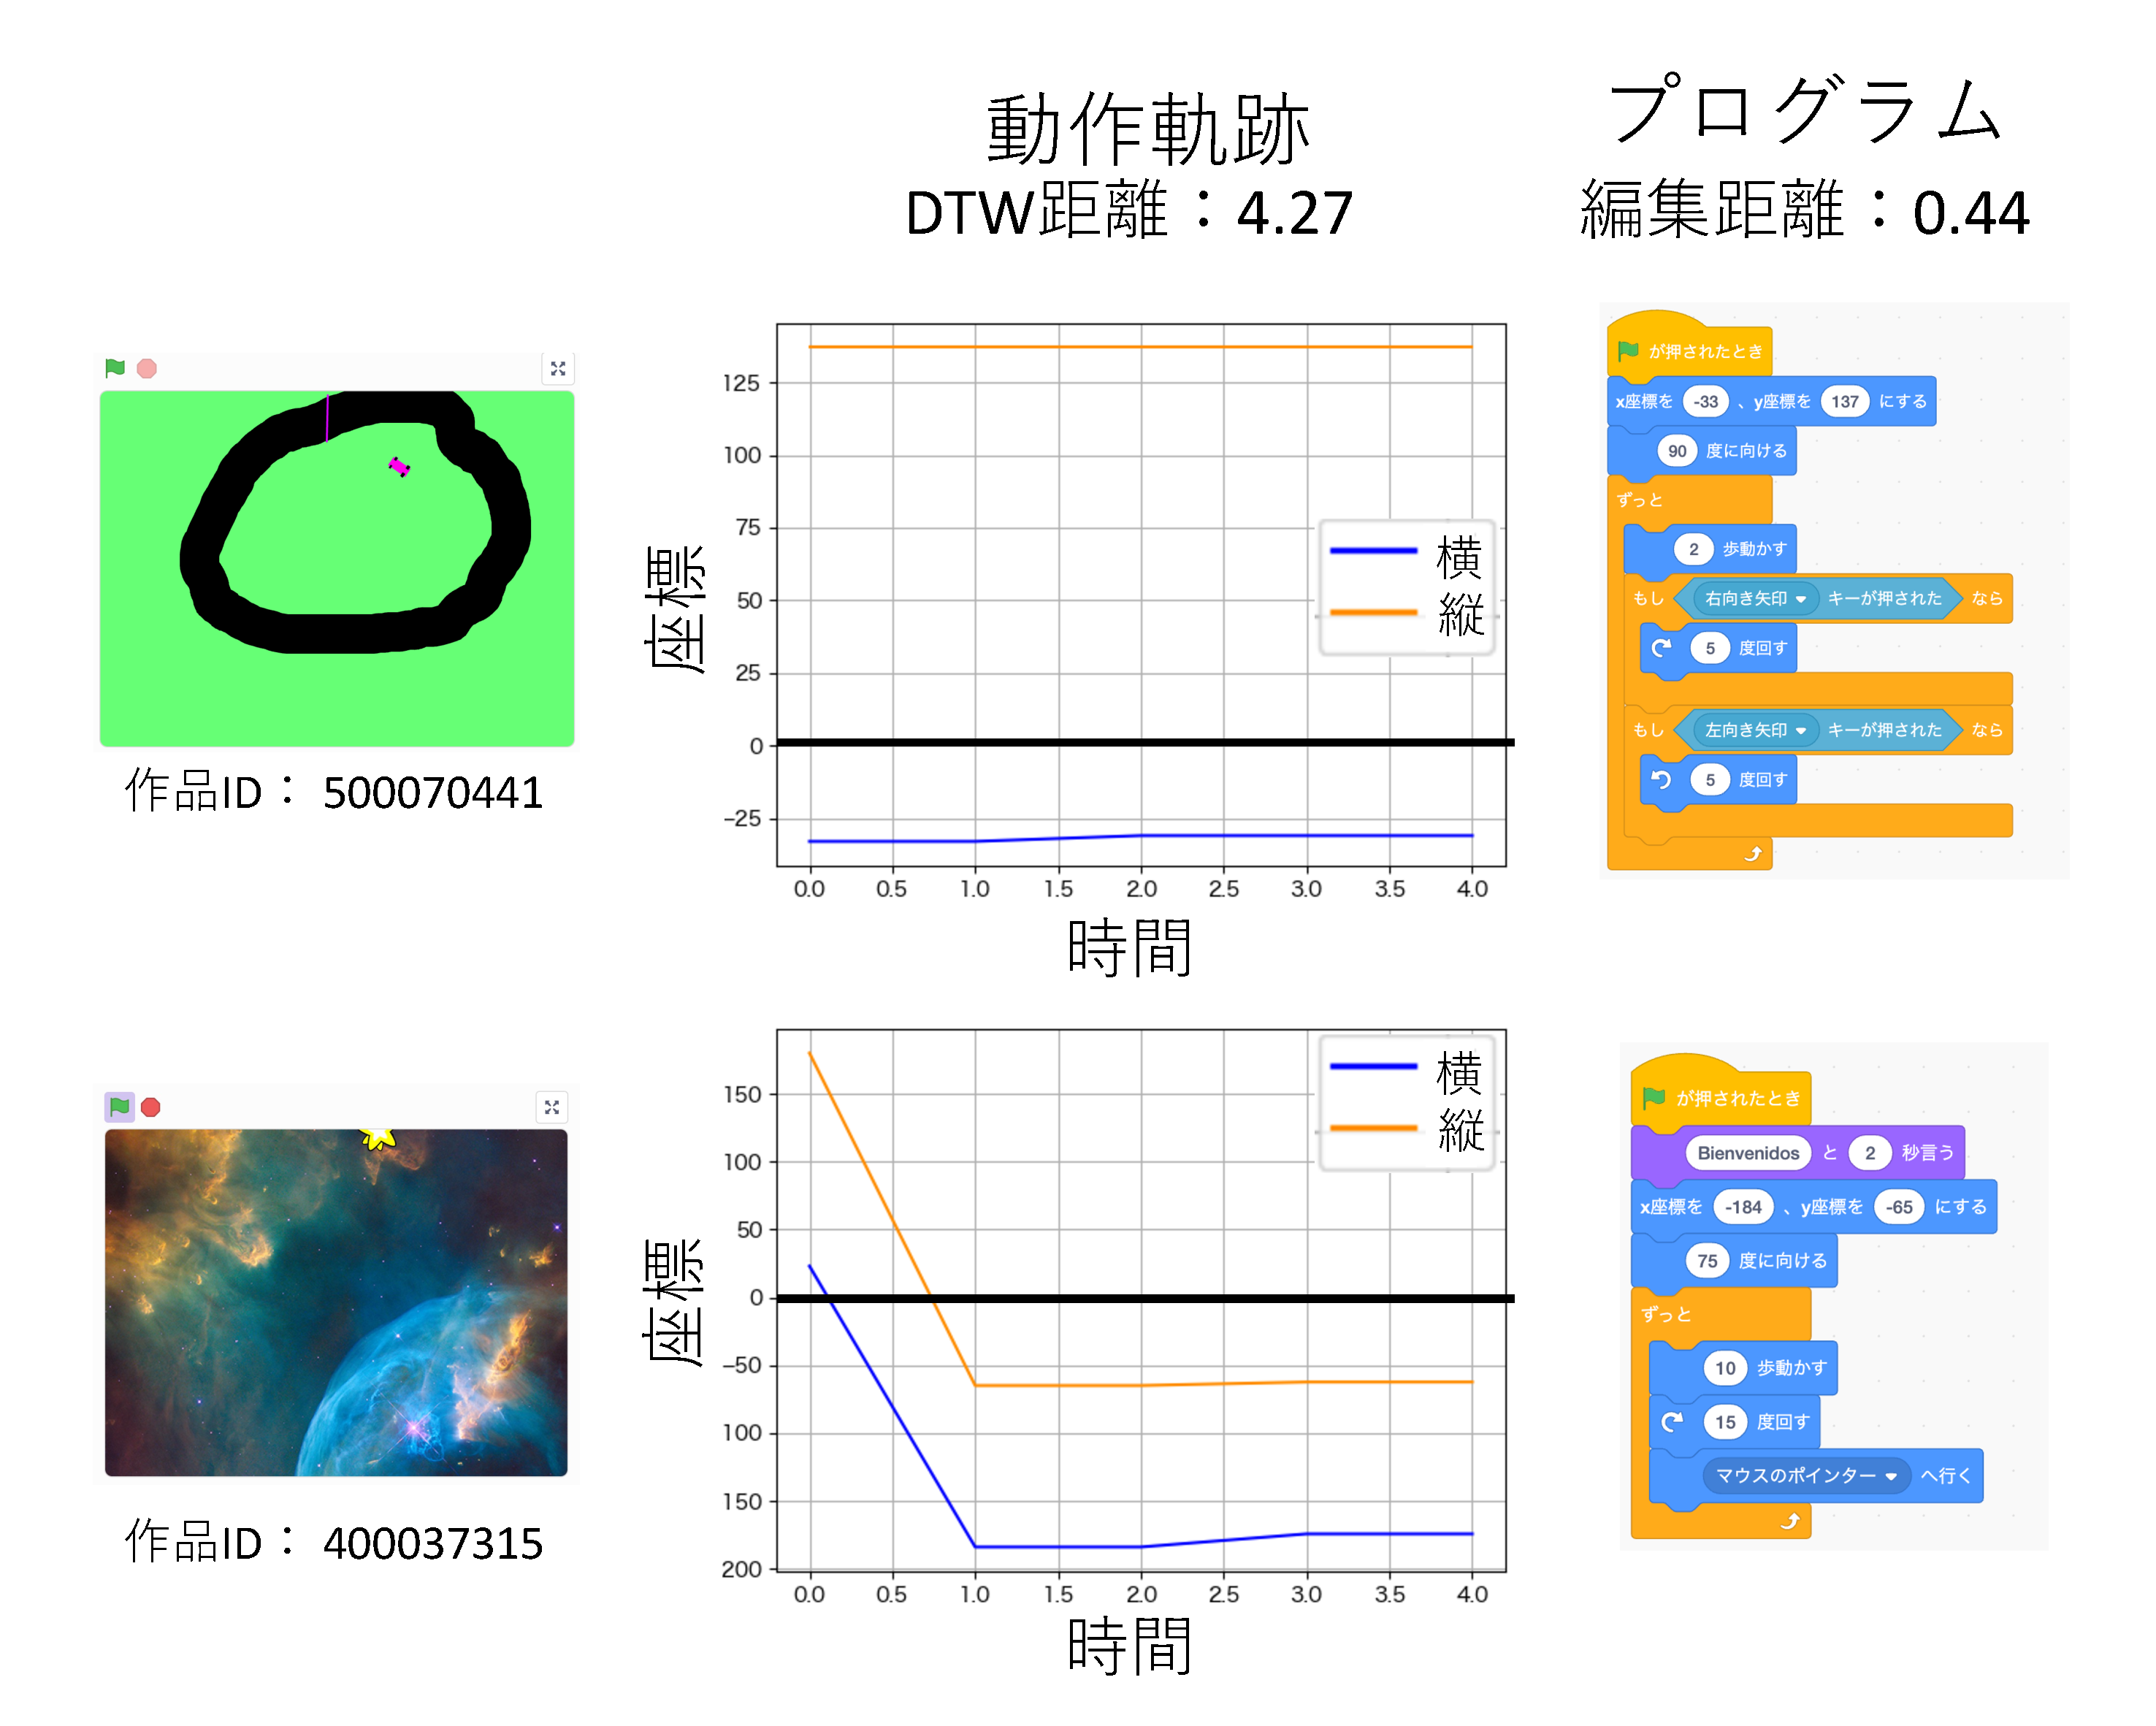
\includegraphics[width=1.0\linewidth]{Okamoto_fig/quadrant-2.pdf}
% 	\caption{DTW距離が4.27,編集距離が0.44の作品対}
% 	\label{fig:distance-boxplot}
% \end{figure}

% % プログラムも動作軌跡も類似する作品対
% \begin{figure}[t]
% 	\centering
% 	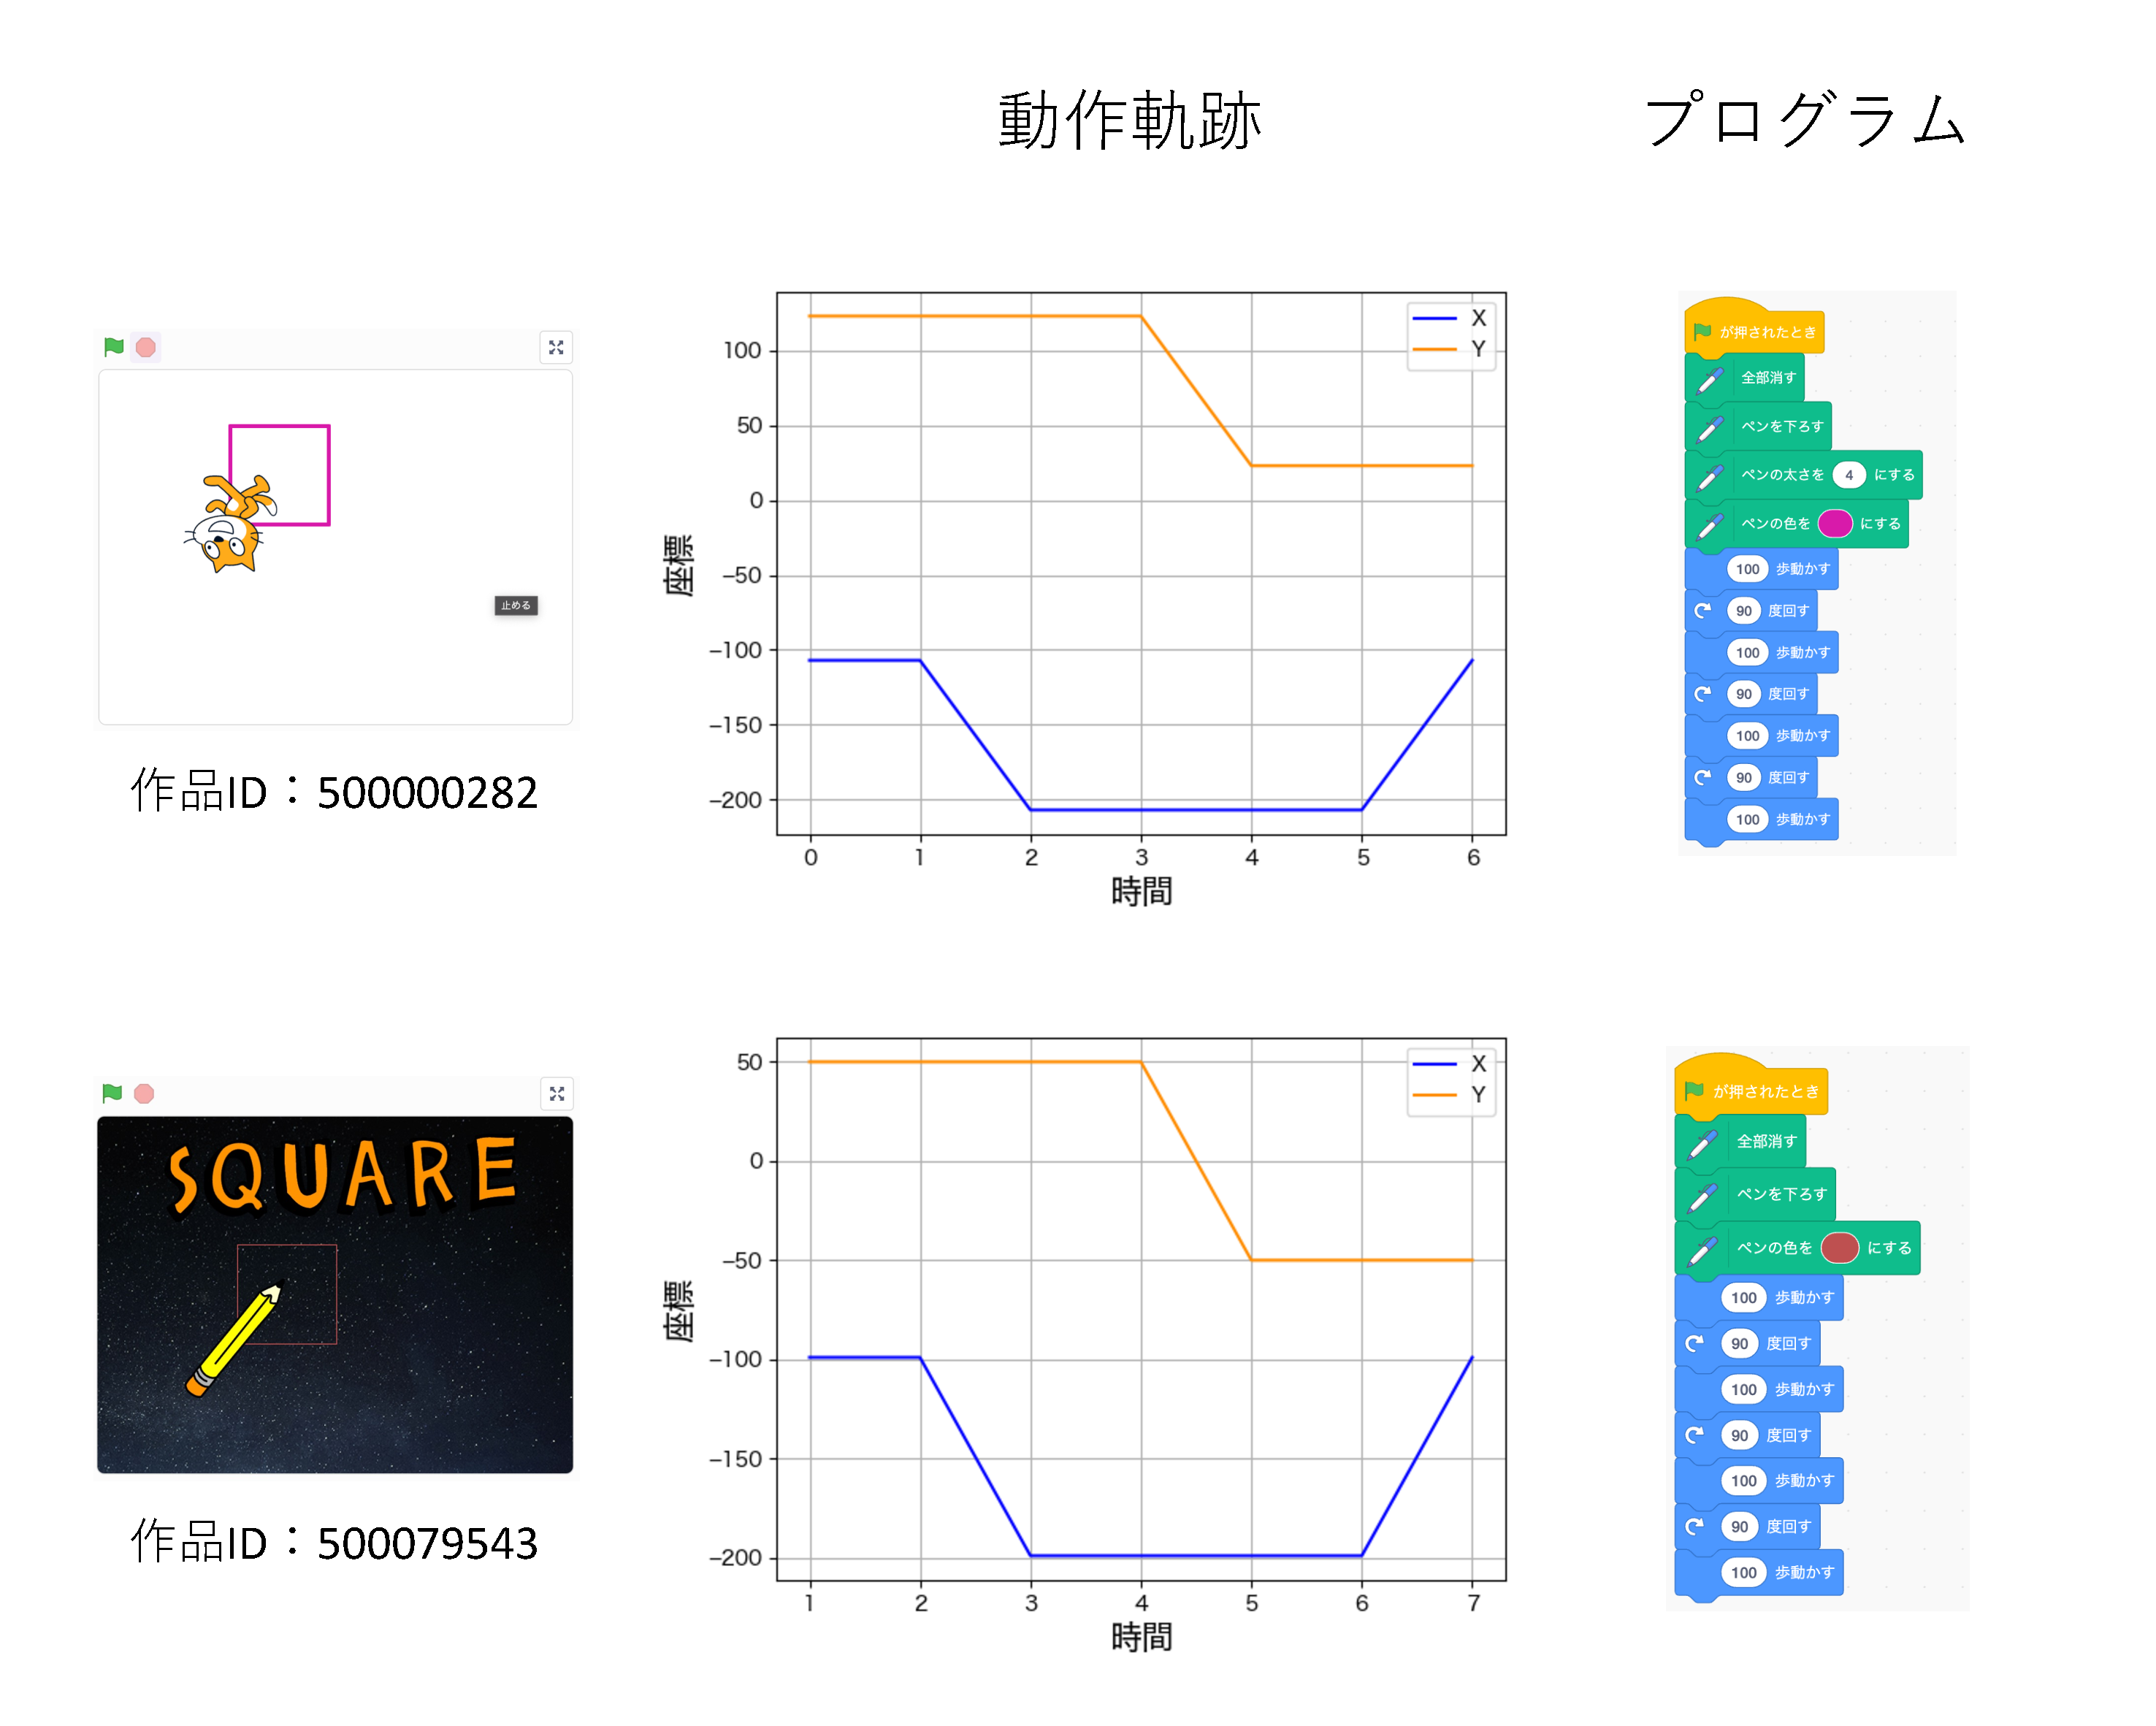
\includegraphics[width=1.0\linewidth]{Okamoto_fig/quadrant-3.pdf}
% 	\caption{DTW距離が1.003e-15,編集距離が0.08の作品対}
% 	\label{fig:distance-boxplot}
% \end{figure}

% % 動作軌跡は類似するが,プログラムは類似しない作品対
% \begin{figure}[t]
% 	\centering
% 	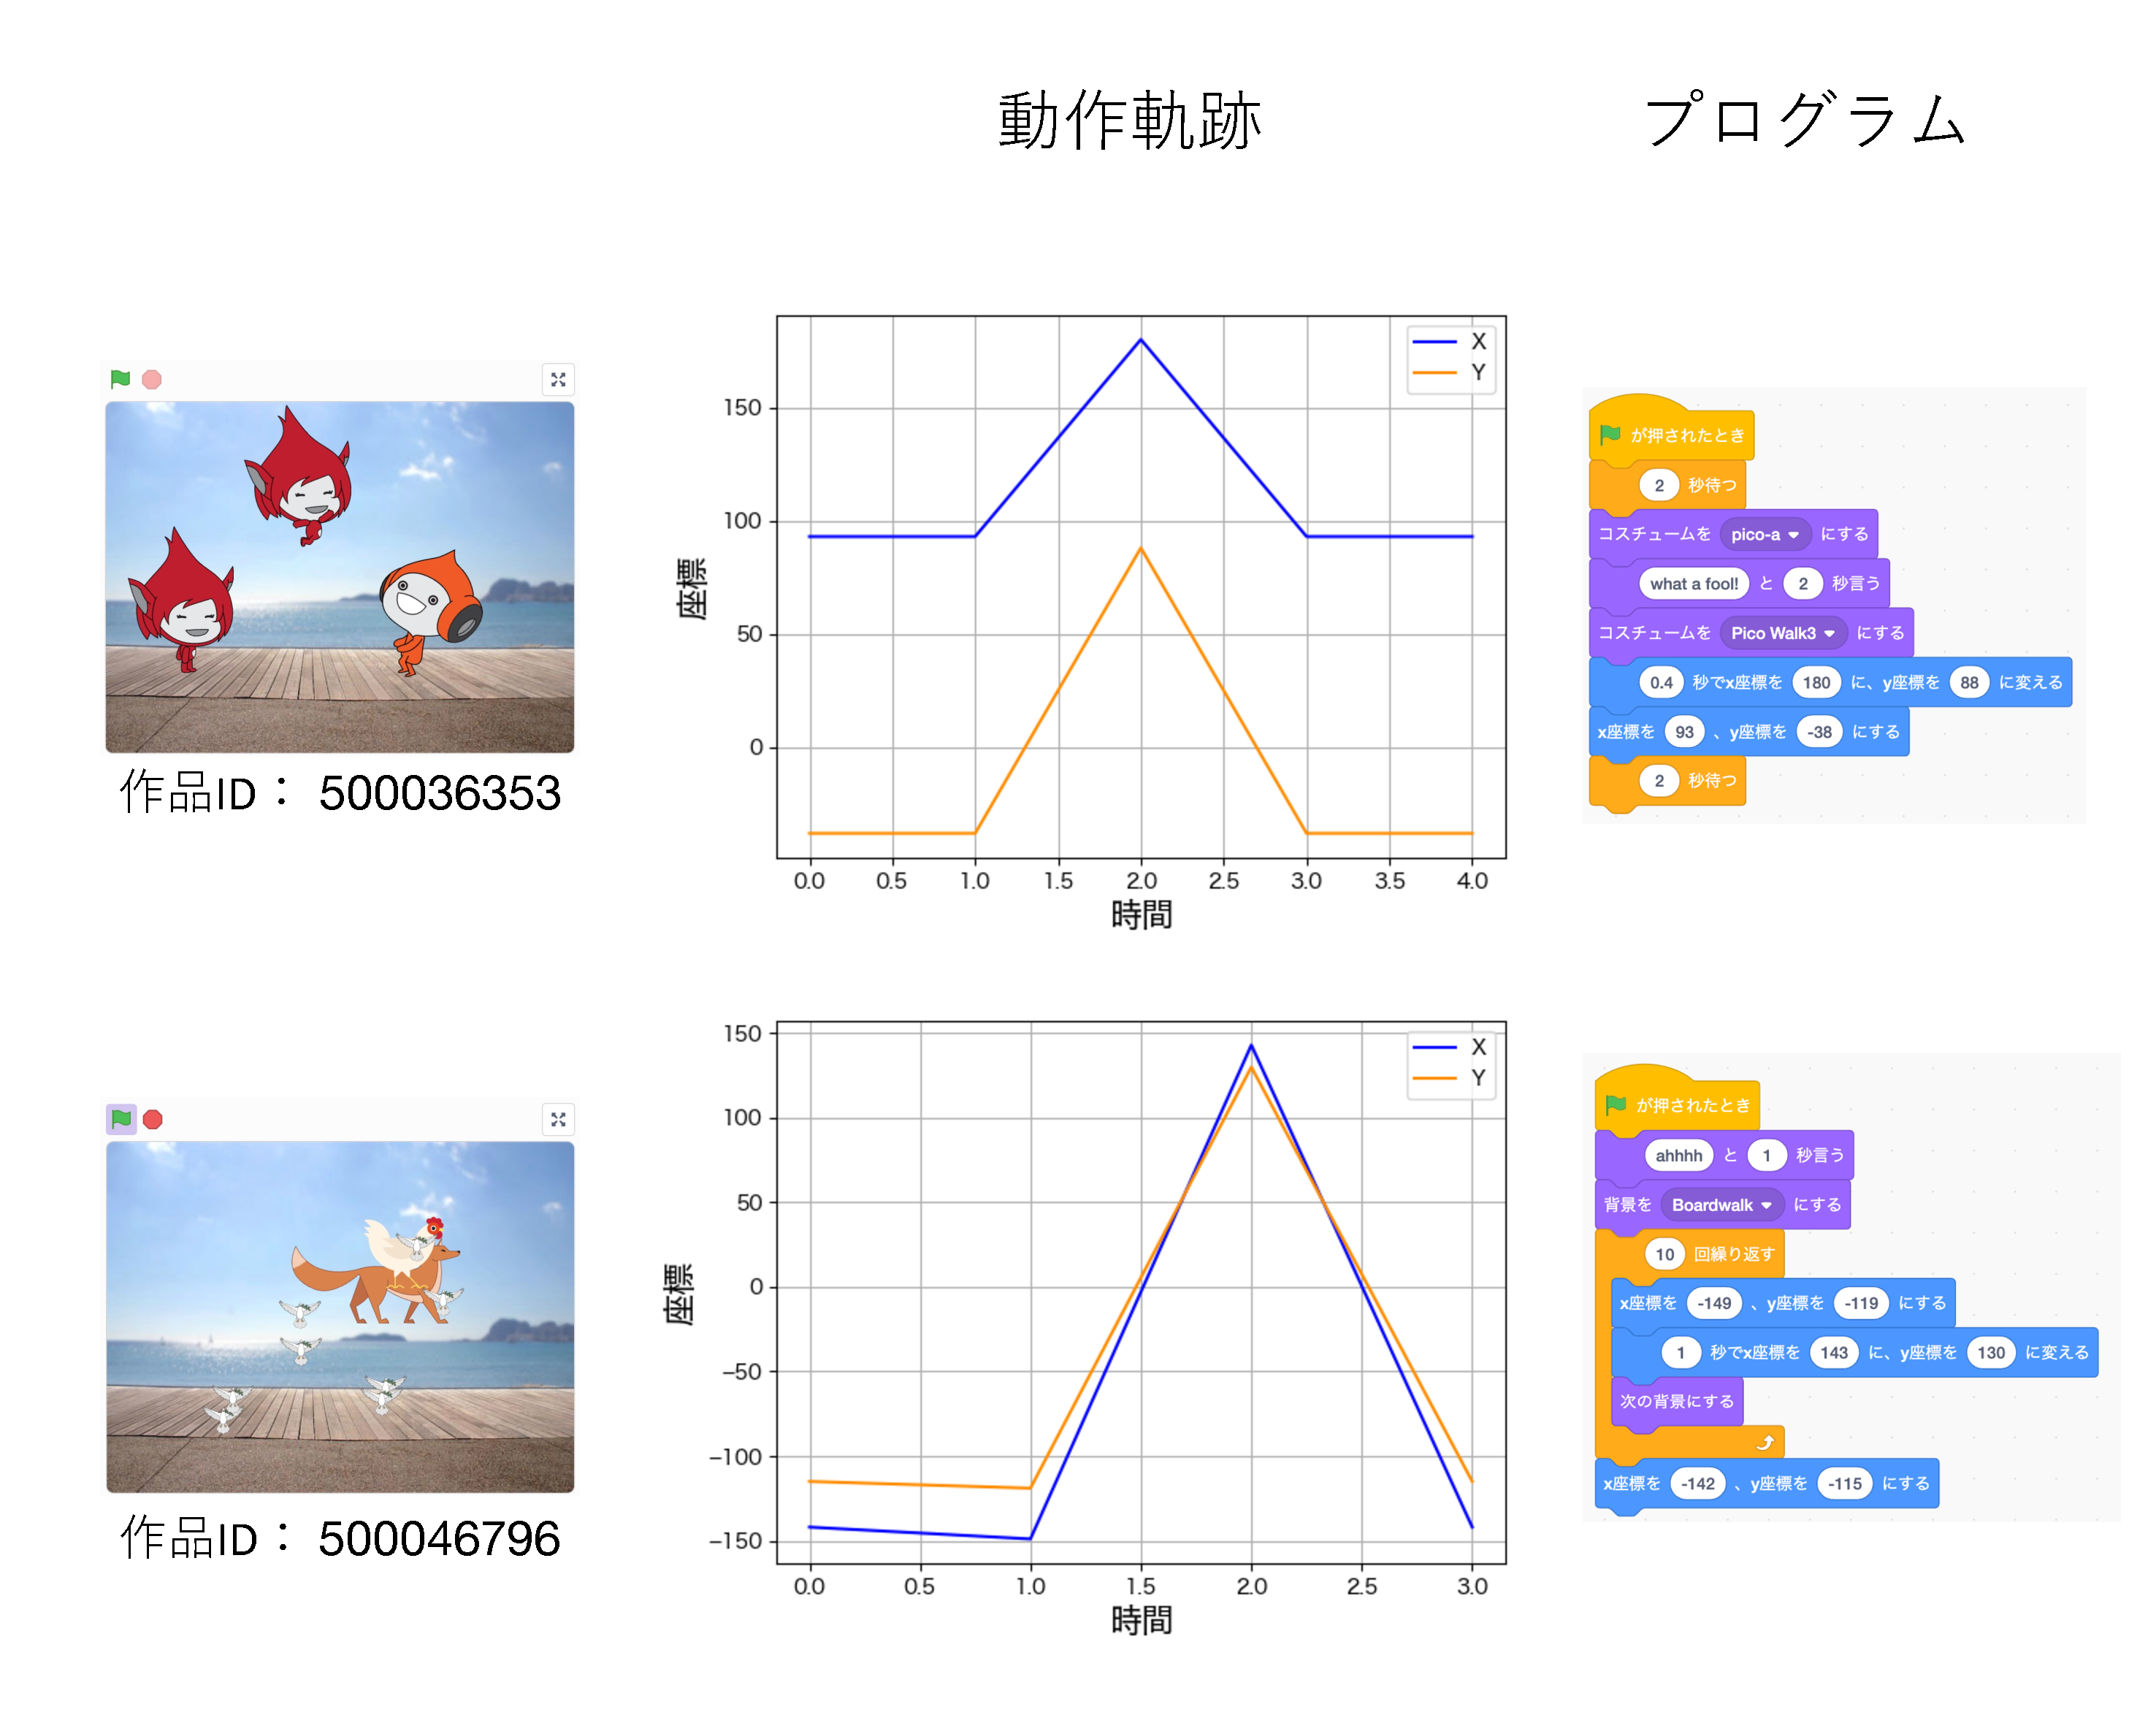
\includegraphics[width=1.0\linewidth]{Okamoto_fig/quadrant-4.pdf}
% 	\caption{DTW距離が0.087,編集距離が0.88の作品対}
% 	\label{fig:distance-boxplot}
% \end{figure}

\subsection{考察}
% 本節では,\ref{subsec:result}の結果を踏まえて,編集距離によるプログラムの類似性の妥当性について考察する.
% 動作軌跡とプログラムのそれぞれについて考察を述べる.
% \subsubsection{動作軌跡の類似性}
% \ref{subsec:result}の結果より,動作軌跡が類似しない作品対が全体の半数以上存在することが判明した.このことから,作品全体で動作軌跡を比較しても動作軌跡が類似しない作品が多くあることがわかる.そのため,動作軌跡を部分的に切り取って類似性を測定することで,動作軌跡が類似する作品対が増加することが示唆される.
% \subsubsection{プログラムの類似性}
本節では,\ref{subsec:result}の結果より,動作軌跡が類似していても,プログラムが類似しない作品対が多く存在するため,編集距離によるプログラムの類似性の妥当性について二つの事例を挙げて考察する.

図\ref{fig:distance-boxplot4}は,動作軌跡が類似してもプログラムが類似しなかった事例を示す.この作品対のプログラムは,それぞれ同じブロックを多く使用しているが,ループの使用有無によりプログラムの構造が異なる.また,図\ref{fig:pattern2-1}は,動作軌跡が類似してもプログラムが類似しなかった事例を示す.この作品対のプログラムは,それぞれ制御文を利用しているためプログラム構造は類似しているが,(2)のプログラムでは座標移動に関わるブロック以外のブロックも多数使用しているため,プログラムが類似していないという結果となった.

これらの課題を解決するために,ブロックを抽象化することによって類似するプログラムを持つ作品を抽出できる.具体的には次の3種類の抽象化の方法を提案する.
\begin{itemize}
    \item \textbf{意味が類似するブロックの抽象化: }座標移動ブロックやif文といった,類似する命令処理を持つブロックを同一のブロックとして扱う.
    \item \textbf{命令タイプが類似するブロックの抽象化: }意味が類似するブロックの抽象化に加えて,同じ命令を実装できずとも,命令タイプが類似しているブロックを同一のブロックとして扱う.例えば,「スプライトが話す」ブロックと「スプライトが考える」ブロックは,スプライトから吹き出しが出て任意の言葉を出力するという点で類似しているため,同一とみなす.
    \item \textbf{動作・制御ブロック以外のブロックの抽象化: }座標移動ブロックと制御ブロック以外のブロック以外を同一とみなすことで,編集距離の値がどのように変化するか調査する.また,座標移動ブロックと制御ブロックについては,命令タイプが類似するブロックの抽象化を行う.
\end{itemize}

% 結果として,動作・制御ブロック以外の抽象化を行った時に最も分類の精度が良くなったが,動作ブロックと制御ブロックを基準にしており,一般化に向けて適切とは言えないため,最終的にその次に精度が高かった意味が類似するブロックの抽象化を最適な抽象化手法とした.

動作ブロックと制御ブロック以外のブロックを抽象化しても動作軌跡に影響はないため,動作軌跡の類似度とプログラムの類似度に着目している本研究では動作・制御ブロックの抽象化することでプログラムの類似性が向上すると示唆する.ただし,抽象化することにより実装の多様性が失われることが考えられるため,プログラムの類似性を向上しつつ,実装の多様性が失われない適切な抽象化手法を今後の研究で検討する.




%%%%%%%%%%%%%%%%%%%%%%%
\section{おわりに}\label{sec:con}
%%%%%%%%%%%%%%%%%%%%%%%

本研究では,Scratchにおいて制作されるプログラムの類似度の測定手法,およびオブジェクト動作軌跡の類似度の測定手法を提案し,ケーススタディとして4,000件のScratch作品を対象に,プログラムが類似するか否か,オブジェクト動作軌跡が類似するか否かの4種類に分類した結果,プログラムは類似するがオブジェクト動作軌跡が類似しない作品は全体の約1\%,オブジェクト動作軌跡は類似するがプログラムが類似する作品は全体の約28\%存在することを確認し,このことから動作軌跡が類似し,プログラムが多様な作品が多いことを明らかにした.また,動作軌跡の類似度とプログラムの類似度が乖離する作品の特徴も事例から明らかにした.今後は,プログラムを抽象化することで,動作軌跡とプログラムがどちらも類似する作品対の数が増加するかを分析し,類似する動作軌跡に対して,実装パターンを明らかにする.d

% \textbf{謝辞}\
% ありがとうございます
% \todo{謝辞}


%\begin{adjustvboxheight} % needed only when Appendix follows
\bibliographystyle{junsrt}
\bibliography{okamoto}

%\end{adjustvboxheight} % needed only when Appendix follows

% 以下はbibtexを使用しない場合の例です.
% 332行目と333行目をコメントアウトしてから使用してください.
% なお,この例では年数順に文献が並んでいるので適切な並び順ではありません.
%\begin{adjustvboxheight} % needed only when Appendix follows
%\begin{thebibliography}{9}
%\bibitem{fose2021} 名倉 正剛,関澤 俊弦 編:ソフトウェア工学の基礎28,日本ソフトウェア科学会{\em FOSE2021}, 近代科学社, 2021.
%\bibitem{fose2022} 角田 雅照,まつ本 真佑 編:ソフトウェア工学の基礎29,日本ソフトウェア科学会{\em FOSE2022}, 近代科学社, 2022.
%\bibitem{fose2023} 吉田 則裕,槇原 絵里奈 編:ソフトウェア工学の基礎30,日本ソフトウェア科学会{\em FOSE2023}, 近代科学社, 2023. (to appear)
%\end{thebibliography}
%\end{adjustvboxheight} % needed only when Appendix follows

%以下は付録の例です.必要ならコメントアウトして使用してください.
%なお,その際には参考文献の前後にある adjustvboxheight 環境のコメントアウトを解除してください.
%\appendix
%\section{付録A} 
%これは付録の例です.

\end{document}


